\documentclass{article}
\usepackage[utf8]{inputenc}
\usepackage{geometry}
\usepackage{longtable}
\usepackage{graphicx} % For including images
\usepackage{hyperref} % For hyperlinks
\usepackage{enumitem}
\usepackage{graphicx}
\usepackage{booktabs} % For professional looking tables
\usepackage{float} % For improved control over floating environments
\usepackage{array}
\usepackage{makecell} % Allows for line breaks within table cells
\usepackage[table]{xcolor} % For cell coloring
\usepackage{tabularx} % Load the package
\usepackage{multirow}
\definecolor{changeColor}{RGB}{220, 220, 220} % Light gray color for changes
\newcommand{\userStoryOne}{\textbf{User Story 1:} As a frequent traveler, I want to subscribe to a comprehensive monthly pass that includes all three networks so that I can save money on my regular commutes.}
\newcommand{\userStoryTwo}{\textbf{User Story 2:} As a passenger, I want to be able to check the balance of my multi-network travel card online so that I can easily manage my travel expenses.}
\newcommand{\userStoryThree}{\textbf{User Story 3:} As a passenger with a subscription, I want to receive automatic notifications about my subscription renewal and any discounts or promotions available so that I can take advantage of cost savings.}
\newcommand{\userStoryFour}{\textbf{User Story 4:} As a tech-savvy passenger, I want to use a mobile app to manage my subscriptions, make payments, and receive digital tickets so that I can have a paperless and convenient travel experience.}
\newcommand{\userStoryFive}{\textbf{User Story 5:} As a passenger interested in sustainability, I want the system to track my travel carbon footprint and offer carbon offset options so that I can make environmentally responsible travel choices.}
\newcommand{\userStorySix}{\textbf{User Story 6:} As a passenger with mobility challenges, I want the payment system to provide information on accessible services and allow for easy purchase of accessible seating across all networks so that I can travel comfortably and safely.}
\newcommand{\userStorySeven}{\textbf{User Story 7:} As an advocate for accessibility, I want the system to offer voice-activated features and screen reader compatibility for passengers with visual impairments so that the service is inclusive and accessible to everyone.}
\newcommand{\userStoryEight}{\textbf{User Story 8:} As an elder, I want a simple interface, so that I don't have to get help to buy tickets.}
\newcommand{\userStoryNine}{\textbf{User Story 9:} As a tourist, I want to choose among many languages, so that I don't have to translate using my phone.}
\newcommand{\userStoryTen}{\textbf{User Story 10:} As a tourist, I want to have quick access to the most popular trips, so I can quickly get my ticket.}
\newcommand{\userStoryEleven}{\textbf{User Story 11:} As a student, I want to be able to scan my student card, so that I can access financial benefits.}
\newcommand{\userStoryTwelve}{\textbf{User Story 12:} As a commuting worker/student, I want a single transaction to get all the subscriptions I need, so that I can travel from home to work/school every day.}
\newcommand{\userStoryThirteen}{\textbf{User Story 13:} As a family, we want to charge train cards from the terminal, so that we can travel when we need without one transaction every time.}
\newcommand{\userStoryFourteen}{\textbf{User Story 14:} As a visually impaired person, I want a high contrast interface and big font, so that I can avoid mistakes when buying my tickets.}
\newcommand{\userStoryFifteen}{\textbf{User Story 15:} As an occasional passenger, I want the system to not allow me to pay for temporarily blocked routes, so that I don't have to go through customer service.}
\newcommand{\userStorySixteen}{\textbf{User Story 16:} As a passenger, I want to be able to purchase a single ticket that allows me to travel across all train networks so that I can travel seamlessly without needing to buy separate tickets for each network.}
\newcommand{\userStorySeventeen}{\textbf{User Story 17:} As a student/commuter, I want the system to tell me which subscriptions I need to go from home to school/work, so that I can get the best price.}
\newcommand{\userStoryEighteen}{\textbf{User Story 18:} As a government regulator, I want the payment system to adhere to data protection and financial transaction security standards so that passengers' personal and financial information is secure.}
\newcommand{\userStoryNineteen}{\textbf{User Story 19:} As a government entity, I want the system to provide detailed reporting on passenger numbers and revenue for each network so that we can assess the public transportation system's efficiency and fairness.}
\newcommand{\userStoryTwenty}{\textbf{User Story 20:} As a local government official, I want to ensure that the payment system includes options for reduced fares for eligible populations (students, elderly, low-income) across all networks so that public transportation is accessible to everyone. Also, as a local government, I want to get usage data from the system, so that I can do urban planning properly.}
\newcommand{\userStoryTwentyOne}{\textbf{User Story 21:} As a tycoon, I want the payment system to accurately track revenue from shared and exclusive segments of my network so that revenue sharing among tycoons is fair and transparent.}
\newcommand{\userStoryTwentyTwo}{\textbf{User Story 22:} As a tycoon, I want the ability to offer exclusive promotions and discounts to passengers using my network to encourage loyalty and increase ridership.}
\newcommand{\userStoryTwentyThree}{\textbf{User Story 23:} As a tycoon, I want the payment system to integrate with my existing infrastructure with minimal disruption so that I can maintain high service levels during the transition.}
\newcommand{\userStoryTwentyFour}{\textbf{User Story 24:} As a tycoon, I want to access analytics and data insights from the payment system to understand passenger behavior and adjust my services accordingly to maximize revenue and improve service.}
\newcommand{\userStoryTwentyFive}{\textbf{User Story 25:} As a station staff member, I want a simple and fast way to assist passengers with ticket purchases and inquiries across all networks so that I can provide efficient customer service.}
\newcommand{\userStoryTwentySix}{\textbf{User Story 26:} As a maintenance team member, I want the system to allow for temporary fare adjustments or bypass options during maintenance work so that we can minimize inconvenience to passengers.}
\newcommand{\userStoryTwentySeven}{\textbf{User Story 27:} As a network maintenance planner, I want the payment system to integrate with maintenance scheduling tools so that I can plan work with minimal disruption to the train service and revenue.}
\newcommand{\userStoryTwentyEight}{\textbf{User Story 28:} As a government financial auditor, I want the payment system to include audit trails and compliance reporting features so that we can ensure transparency and accountability in revenue management.}
\newcommand{\userStoryTwentyNine}{\textbf{User Story 29:} As the TrIP owner, I want the system to operate with the lowest possible operational costs, so that it remains cost-effective over time.}
\newcommand{\userStoryThirty}{\textbf{User Story 30:} As the TrIP owner, I want the system maintenance efforts to be easily scalable, so that costs do not increase disproportionately as we expand.}
\newcommand{\userStoryThirtyOne}{\textbf{User Story 31:} As the TrIP owner, I want routine maintenance tasks to be automated, so that manual labor and operational costs are reduced.}
\newcommand{\userStoryThirtyTwo}{\textbf{User Story 32:} As the TrIP owner, I want a cost-effective database solution for data management, so that storage and access costs remain low.}
\newcommand{\userStoryThirtyThree}{\textbf{User Story 33:} As the TrIP owner, I want an efficient error handling and reporting mechanism, so that system downtime is minimized and maintenance is cost-effective.}
\newcommand{\userStoryThirtyFour}{\textbf{User Story 34:} As the TrIP owner, I want to implement energy-efficient and eco-friendly technologies, so that the system's operational costs are sustainable and environmentally friendly.}
\newcommand{\userStoryThirtyFive}{\textbf{User Story 35:} As a new tycoon entering the market, I want to easily integrate my services with the TrIP system, so that passengers can quickly benefit from additional travel options.}
\newcommand{\userStoryThirtySix}{\textbf{User Story 36:} As a system administrator, I want the ability to add and configure services from new tycoons without significant downtime, so that the system remains up-to-date and competitive.}
\newcommand{\userStoryThirtySeven}{\textbf{User Story 37:} As a passenger, I want to see new transportation options as soon as they become available, so that I can plan my trips with the most comprehensive information.}
\newcommand{\userStoryThirtyEight}{\textbf{User Story 38:} As a tycoon, I want my data (such as timetables, prices, and updates) to be accurately and promptly reflected in the system.}
\newcommand{\userStoryThirtyNine}{\textbf{User Story 39:} As a passenger, I expect ticket validation to work seamlessly, even during network outages, ensuring that my travel is not hindered by technical issues.}
\newcommand{\userStoryForty}{\textbf{User Story 40:} As a tycoon, I require the system to handle all transactions securely and efficiently, irrespective of the current network status, to maintain service continuity and safeguard revenue.}
\newcommand{\userStoryFortyOne}{\textbf{User Story 41:} As the TrIP owner, I want to use a service-based architecture, so that the system is easy to maintain and update.}
 

\geometry{
 a4paper,
 total={170mm,257mm},
 left=20mm,
 top=20mm,
}

\title{Software Architecture of Train Inter Payment System (TrIP)}
\author{Group 04}
\date{\today}

\begin{document}

\maketitle
\newpage

\tableofcontents
\newpage

\section{Introduction}
The Train Inter Payment System (TrIP) is a collaborative project initiated by three railroad tycoons to streamline the payment process for train travel. These tycoons, operating a network connecting towns, industries, and a university, aim to address the interoperability issues of their existing payment systems. TrIP will feature smart payment terminals at each station, enabling direct communication for subscription validation or single-fare payments. This system, underpinned by a service-based architecture, involves critical components like payment terminals and tycoon-specific systems. It's designed with key stakeholder requirements in mind: maintainability and operational efficiency for the owner, usability and reliability for the tycoons, and usability and security for passengers. The project seeks to ensure passengers can easily manage payments and subscriptions across the network, enhancing the overall travel experience while safeguarding passengers data.
\newpage

\section{Decisions}
\subsection{Decision 1: User Interface}

\subsection*{Status}
Accepted. 
Reviewed after the decision to include a smartphone application and a web application.

\subsection*{Architectural Summary}
\begin{tabular}{|p{3.5cm}|p{10.5cm}|}
    \hline
    \textbf{In the context of} & Designing a user interface for the TrIP system payment terminals \\
    \hline
    \textbf{Facing} & The challenge of letting various type of passengers easily find information and make purchases, \\
    \hline
    \textbf{To achieve} & A seamless experience that is intuitive, accessible, and responsive, and maintains the system's usability and passenger satisfaction \\
    \hline
    \textbf{We considered} & Option 1: Use of Standardized UI Components; Option 2: Custom Designed Interactive Interfaces; Option 3: Open Source Frameworks; Option 4: Proprietary High-End Frameworks \\
    \hline
    \textbf{And decided for} & Option 1: Use of Standardized UI Components \\
    \hline
    \textbf{Because} & It offers a balance of development speed, consistency, and usability that meets our criteria and constraints \\
    \hline
    \textbf{Accepting} & Potential dependency on external communities and companies. \\
    \hline
\end{tabular}

\subsection*{Concern}
Passengers require a user interface that is easy to navigate, visually appealing, and provides a seamless experience across different tycoon systems.
we face the challenge of selecting guiding principles and frameworks that will shape the user experience and interaction design.
Related user stories are listed here:

\begin{itemize}
    \item \textbf{User Story 16:} As a passenger, I want to be able to purchase a single ticket that allows me to travel across all train networks so that I can travel seamlessly without needing to buy separate tickets for each tycoon's network.
    \item \textbf{User Story 7:} As an advocate for accessibility, I want the system to offer voice-activated features and screen reader compatibility for passengers with visual impairments so that the service is inclusive and accessible to everyone.
    \item \textbf{User Story 14:} As a visually impaired person, I want a high contrast interface and big font, so that I can avoid mistakes when buying my tickets.
    \item \textbf{User Story 9:} As a tourist, I want to choose among many languages, so that I don't have to translate using my phone.
\end{itemize}

\subsection*{Context}
We need to design an intuitive and engaging user interface for the TrIP system terminals, web application and smartphone application.
The design of the user interface on the terminals involves the passenger's interaction with the system, from querying routes to finalizing ticket purchases.

\subsection*{Criteria}
The decision will be guided by the following criteria:
\begin{itemize}
    % TODO:mention usability
    \item Consistency in design to provide a unified look and feel across all terminals, web apps and smartphone apps.
    \item Accessibility to ensure the system is usable by all passengers, including those with disabilities.
    \item Responsiveness so that the interface can adapt to various screen sizes and orientations.
    \item Ease of maintenance and scalability for future enhancements.
    \item Alignment with the latest trends in user interface design and technology.
\end{itemize}

\subsection*{Option 1: Use of Standardized UI Components}
This approach involves adopting a comprehensive design system, such as Google's Material Design or IBM’s Carbon Design System, which offers a robust set of standardized UI components. These components include buttons, forms, toggles, navigation patterns, and more, all designed with consistency and usability in mind. By utilizing these pre-designed components, the development process can be significantly accelerated, as developers and designers will not need to create common UI elements from scratch. This ensures a cohesive look and feel across the entire application, enhancing the user's ability to intuitively navigate the system.
\begin{itemize}
    \item \textbf{Pro:} Significantly reduces development time and ensures UI consistency.
    \item \textbf{Pro:} Both Google's Material Design and IBM's Carbon Design System are open source, hence they would allow developers to easily debug the interface, identify possible bugs, seek for contributions online or even contribute themselves.
    \item \textbf{Con:} May limit unique branding opportunities and design customization. 
    \item \textbf{Con:} Some developers may consider it a limit for their creativity. 
\end{itemize}

\subsection*{Option 2: Custom Designed Interactive Interfaces}
This option focuses on creating bespoke interactive interfaces from the ground up, specifically tailored to the unique needs and brand identity of the TrIP system. This could involve developing custom animations, unique layout designs, and interactive elements that engage users in a novel way. By focusing on custom designs, the TrIP system can distinguish itself from competitors and provide a unique user experience that directly addresses specific user needs and preferences.
\begin{itemize}
    \item \textbf{Pro:} Allows for full creative freedom and the opportunity to innovate.
    \item \textbf{Pro:} Less operational cost, and higher maintainability.
    \item \textbf{Con:} More time-consuming and expensive due to the bespoke nature of the design and development process.
    \item \textbf{Con:} Expertise within the developing team is needed, possibly more developers. This might offset the lower operational cost.
\end{itemize}

\subsection*{Option 3: Open Source Frameworks}
Utilizing open-source UI frameworks such as Bootstrap, Foundation, or Vue.js offers a middle ground between complete customization and strict standardization. These frameworks are supported by large communities of developers, ensuring that the frameworks are well-documented, frequently updated, and robust against common web development challenges. They come with a variety of UI components that can be easily modified to fit the system’s needs, providing both speed in development and a degree of customization.
\begin{itemize}
    \item \textbf{Pro:} Combines rapid development with the flexibility of customization.
    \item \textbf{Con:} Might still require significant effort to stand out from the default "framework look."
    \item \textbf{Con:} Possible discontinuation.
\end{itemize}

\subsection*{Option 4: Proprietary High-End Frameworks}
Choosing proprietary frameworks such as Telerik, DevExpress, or Adobe XD’s design systems offers access to a suite of advanced features, including sophisticated data visualization tools, complex UI components, and comprehensive support services. These frameworks are often optimized for performance and come with extensive documentation and professional support, ensuring that the development team can create a high-quality user interface while potentially saving time on troubleshooting and problem-solving.
\begin{itemize}
    \item \textbf{Pro:} Provides a wide range of advanced features and dedicated support.
    \item \textbf{Con:} Incurs additional costs due to licensing fees and may lock the project into a specific vendor or technology stack.
    \item \textbf{Con:} Train system doesn't have to be that compilicated, high-end products can be redundant, also the passengers want us to keep it simple.
\end{itemize}

\subsection*{Decision}
Option 1 is chosen. This option lifts a lot of weight from the development team. This reduces operational cost and enhances maintenability, which are the main concerns of the TrIP owner. Furthermore, these interfaces are well tested and user-friendly, making them a natural choice to satisfy the need for usability of the passengers and the reliability requested by the tycoons. 
Generally speaking, user interfaces for train systems are not sophisticated enough to require more expensive and complicated set-ups. 
A careful user testing is strongly adviced, to choose a suitable setup.

\subsection*{Consequences}
\textbf{Positive Consequences:}
\begin{itemize}
    \item Access to a broad community for support and troubleshooting.
    \item Cost savings by avoiding licensing fees associated with proprietary software.
    \item Rich ecosystem of plugins and extensions to enhance functionality.
    \item Frequent updates and a large pool of developers familiar with the frameworks.
\end{itemize}
\textbf{Negative Consequences:}
\begin{itemize}
    \item Potential dependency on external communities for critical updates and support. Some of these might require expensive professional support.
    \item Risk of choosing a framework that may not align with long-term technology trends or become obsolete. Information sourcing about the future of the chosen project is crucial.
    \item Need for rigorous selection to ensure accessibility and responsiveness standards are met. This would be a consequence of any of the choices listed.
\end{itemize}


\newpage
\subsection{Decision 2: Routes management}

\subsection*{Status}
Accepted.

\subsection*{Architectural Summary}
\begin{tabular}{|p{3.5cm}|p{10.5cm}|}
    \hline
    \textbf{In the context of} & Allowing terminals to present route options to passengers when they select their departure and arrival stations, \\
    \hline
    \textbf{Facing} & The challenge of letting passengers choose between different travel combination involving multiple tycoons, \\
    \hline
    \textbf{To achieve} & Integration with multiple tycoon systems, and accurate representation of options based on multiple factors, \\
    \hline
    \textbf{We considered} & Option 1: Direct Tycoon Integration; Option 2: Centralized Route Management Module; \\
    \hline
    \textbf{And decided for} & Option 2: Centralized Route Management Module \\
    \hline
    \textbf{Because} & It simplifies data flow and integration between the TrIP system and tycoon's systems, it improves scalability and maintainability of the system, \\
    \hline
    \textbf{Accepting} & Initial development effort and potential difficulties in data synchronization across modules. \\
    \hline
\end{tabular}

\subsection*{Concern}
The concern is to facilitate a seamless travel planning experience for passengers by ensuring the system can accurately and efficiently gather available route options and present them based on the user's criteria of price, time, and subscription status.
Related user stories are listed here:
\begin{itemize}[noitemsep]
    \item \userStorySixteen,
    \item \userStoryTwentySix,
\end{itemize}

\subsection*{Context}
The TrIP system needs to be able to compute optimized travel options (for instance best prices and lowest travel times), gathering information from multiple tycoon systems in order to align with passenger preferences and existing subscriptions.
The decision is centered on the system's interface with tycoon systems to retrieve and optimize route data, which impacts the functionality and performance of the terminal's route planning features for the passengers.

\subsection*{Criteria}
The key criteria for the decision include:
\begin{itemize}[noitemsep]
    \item \textit{Functionality and usability}: Comprehensive and diverse route options.
    \item \textit{Functionality}: Accurate representation of options based on multiple factors.
    \item \textit{Integrability}: Streamlined integration with multiple tycoon systems.
\end{itemize}

\subsection*{Option 1: Direct Tycoon Integration}
Terminals directly interface with each tycoon system and the central database to collate route options. The route optimizer processes this data to present optimal travel solutions. This requires our system to have APIs to query each of the tycoons systems.
\begin{figure}[ht]
    \centering
    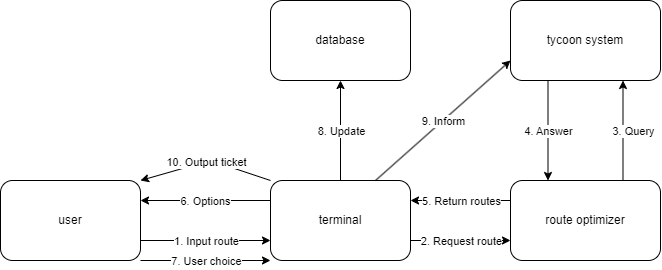
\includegraphics[width=\textwidth]{drawings/decision3_drawings/direct.png}
    \caption{Direct Data Management Interface}
    \label{fig:direct-data-interface}
\end{figure}

\subsection*{Option 2: Centralized Route Management Module}
A central route data management module acts as an intermediary between terminals and tycoon systems, standardizing and aggregating data before it is processed by the route optimizer. A database containing the timetables will be kept up to date by the tycoon (possibly though an API, this will be the focus of a later decision). The route data management system might cache optimized routes, in order to minimize database requests. A module specialized in running optimizations with the data it is provided with interacts solely with the Route Management Module.
\begin{figure}[ht]
    \centering
    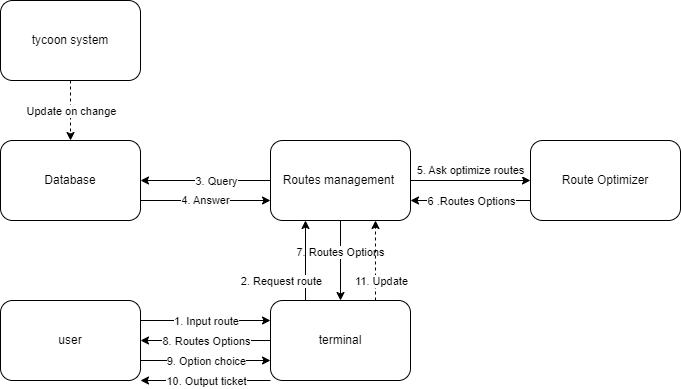
\includegraphics[width=\textwidth]{drawings/decision3_drawings/centralized.png}
    \caption{Centralized Route Management Module. Dashed lines represents steps to be explained in future decisions.}
    \label{fig:centralized-data-interface}
\end{figure}
  
\subsection*{Decision}
We have decided to proceed with Option 2: Centralized Route Management Module. This decision is based on the module's ability to simplify the data flow between systems and to effectively manage the complexity of integrating with multiple tycoon systems. The introduction of a separate data management module will allow for greater flexibility and scalability.

\subsection*{Consequences}
\textbf{Positive Consequences:}
\begin{itemize}
    \item Simplified data flow between the trip system and tycoons.
    \item Improved scalability and maintainability of the system.
    \item Easier to integrate with current and future tycoon systems.
\end{itemize}
\textbf{Negative Consequences:}
\begin{itemize}
    \item Initial development and integration effort for the new module.
    \item Potential complexity in data synchronization between modules.
\end{itemize}
This approach is expected to provide a solid foundation for the system's scalability and adaptability to evolving requirements and stakeholder needs.
\newpage
\subsection{Decision 3: Account and Subscriptions management}

\subsection*{Status}
Accepted. Reviewed to consider Event 1 (tycoon default) and to add the possibility of outsourcing subscription management.

\subsection*{Architectural Summary}
\begin{tabular}{|p{3.5cm}|p{10.5cm}|}
    \hline
    \textbf{In the context of} & managing subscriptions and accounts of passengers, \\
    \hline
    \textbf{Facing} & the challenge of integrating many different subscriptions for the same passenger and letting subscription separated, \\
    \hline
    \textbf{To achieve} & streamlined integration with multiple tycoon systems, high passenger usability, ease of maintenance, \\
    \hline
    \textbf{We considered} & Option 1: Introduction of a subscription manager tool.; Option 2: Integrated Subscription-Route Optimization Service; Option 3: Include a Single-Ticket management module\\
    \hline
    \textbf{And decided for} & Option 1: Introduction of a subscription manager tool; and Option 3: Include a Single-Ticket management module  \\
    \hline
    \textbf{Because} & It enhances scalability and maintainability though modularity, it reduces system-wide failures risks, allows occasional travellers to easily use the system, \\
    \hline
    \textbf{Accepting} & Increased System Complexity, higher Initial Costs, Data Consistency Challenges. \\
    \hline
\end{tabular}

\subsection*{Concern}
A passenger wants to traver around the network using its subscription(s) instead of always having to buy a single fare.
Tycoons have explicitely requested to maintain their own subscriptions separated.
The following user stories are tied to this decision:
\begin{itemize}[noitemsep]
    \item \userStorySixteen,
    \item \userStoryTwentyThree,
    \item \userStoryThirty,
\end{itemize}

Specific concerns identified for the system include the following:
\begin{itemize}
    \item A passenger should be able to have different subscriptions for the three tycoons.
    \item Each of the three tycoon wants to have its own subscription fee system.
\end{itemize}

\subsection*{Context}
In developing the TrIP system, we explore subscription model architectures that align railway tycoons' need for flexibility with passengers' demand for simplicity. 
We assess the trade-offs between unified and tycoon-specific models to enhance both operational autonomy and passenger convenience.
When passengers want to go from station A to station B, they want to be able to use all the subscription they have and pay for the trains belonging to tycoons they are not subsribed to.
The terminal has to communicate with the tycoon systems to verify subscriptions and check routes.
Alternatively, if passengers have active subscriptions to a tycoon, they should be allowed onboard the train without a ticket. 

\subsection*{Criteria}
\begin{itemize}[noitemsep]
    \item \textit{Usability}: Ease of use for the passenger.
    \item \textit{Functionality}: Multiple route and subscriptions options for the passenger without excessive effort.
    \item \textit{Functionality}: The system returns to the passenger usable options based on price/time/availability/subscription.
    \item \textit{Integrability}: Simple integration with the tycoon systems.
    \item \textit{Maintainability and scalability}: Ease to accomodate changes in the subscriptions options from tycoons.
\end{itemize}

\subsection*{Option 1: Introduction of a subscription manager tool, route management needs to take passenger subscriptions into consideration.}
We want to include a Subscription Manager module to our functional view. 
Such a module has the responsibility to verify subscriptions, communicating with the tycoon system.
It should also allow passengers to create their own TrIP account and tie it to subscriptions.
Since we need scalability, we consider using a TrIP account that is tied to one or many subscriptions, and let the passenger add new or automatically renew the existing ones.
This means that we need an authentication means, like a magnetic card, or a phone app linked to NFC scanning or other alternatives.
This will be the topic of a future decision.
Furthermore, the Route management module needs to be able to optimize with respect to price, given that the passenger holds some subscription.
The idea is to add an optional initial iteration to the sequence of actions sketched in decision 3.
This requires a way to communicate the subscription to the terminal, be it a QR code, a code or a magnetic card. 
This should be the topic of another decision.
\begin{figure}[ht]
    \centering
    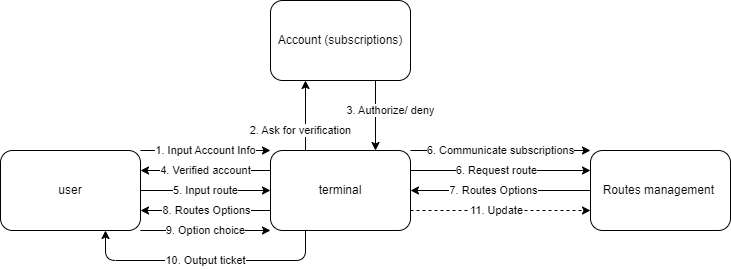
\includegraphics[width=\textwidth]{drawings/decision4_drawings/account_functional.png}
    \caption{Account Management Interaction for single-ticket.}
    \label{fig:account_management_ticket}
\end{figure}
\subsection*{Pros}

\begin{itemize}[noitemsep]
    \item \textbf{Modular Architecture:} The separation of subscription management and route optimization into distinct modules enhances the system's modularity, making it easier to maintain, update, or replace parts of the system without affecting others.
    \item \textbf{Scalability:} Designed with scalability in mind, allowing for easy addition and management of new subscriptions or renewal of existing ones, which can accommodate growing passenger demands and evolving business requirements.
    \item \textbf{Reduced Risk of System-wide Failures:} By distributing functionalities across different systems or modules, the impact of a failure in one component is limited, reducing the risk of system-wide outages and improving overall system reliability.
    \item \textbf{Flexibility in Passenger Authentication:} Supports various means of passenger authentication (e.g., magnetic card, smartphone app), offering flexibility and convenience for passengers to access their subscriptions and travel seamlessly.
\end{itemize}

\subsection*{Cons}

\begin{itemize}[noitemsep]
    \item \textbf{Increased System Interactions:} The decoupled nature of the system requires more interactions between separate modules (e.g., subscription verification and route optimization), which can increase the complexity of integration and potentially lead to higher latency in response times.
    \item \textbf{Integration Complexity:} Ensuring seamless communication and data consistency between different modules can introduce additional complexity in system integration and require more sophisticated coordination mechanisms.
    \item \textbf{Higher Overhead:} Managing separate systems for subscription and route optimization may lead to higher operational overhead in terms of both system resources and administrative efforts to maintain multiple components.
\end{itemize}

\subsection*{Option 2: Integrated Subscription-Route Optimization Service}
The Integrated Subscription-Route Optimization Service (IS-ROS) combines the functionality of subscription management and route optimization into a single service. 
\subsubsection*{Pros}
\begin{itemize}[noitemsep]
    \item \textbf{Performance} Streamlines the process by combining two functionalities, potentially reducing response time for route optimization.
    \item \textbf{Reduced Interactions between systems} Simplifies the architecture by reducing the number of interactions between separate systems.
\end{itemize}
\subsubsection*{Cons}
\begin{itemize}[noitemsep]
    \item \textbf{Increased Complexity within Single Module} Increases complexity within a single system, which may require more resources to develop and maintain.
    \item \textbf{Failures have larger impact} May lead to higher dependency on a single system, which can be a point of failure if the system goes down.
\end{itemize}

\subsection*{Option 3: Include a Single-Ticket management module}
Abstractly, a single ticket can be seen as an account that expires once the journey is completed. As an account, it is linked to a passenger via their personal data, if it is related to a booking or via 
an anonymous user ID if it is not.
Its temporary nature though causes different needs for information storage and flow, as updates for single tickets occurs often.
Hence the need for a separated module and a related database.

\subsection*{Pros}
\begin{itemize}[noitemsep]
    \item Efficient management specific to single-ticket purchases, improving usability for occasional travellers.
    \item Dedicated module enhances system's ability to handle frequent updates inherent to temporary accounts.
    \item Improved usability for less tech-savy passengers.
\end{itemize}

\subsection*{Cons}
\begin{itemize}[noitemsep]
    \item Adds complexity to the system, requiring sophisticated integration with other components.
    \item Potential for fragmented customer experience when navigating between single-ticket and subscription services.
\end{itemize}

\subsection*{Option 4: Complete outsourcing of the subscription management}
The system could be implemented as only taking care of payments, letting some other system or the tycoons themselves tell our system who has which subscription and how subscription changes pricing and rights.

\subsection*{Pros}
\begin{itemize}[noitemsep]
    \item Simplifies the system's responsibilities, focusing on payment processing.
    \item Reduces internal system complexity by leveraging external expertise for subscription management.
    \item Potentially lowers initial development and maintenance costs by relying on tycoons' existing infrastructure.
\end{itemize}

\subsection*{Cons}
\begin{itemize}[noitemsep]
    \item Introduces dependencies on external systems, potentially affecting reliability and response times.
    \item Limits control over the subscription management experience, impacting the ability to implement customized features.
    \item Raises integration challenges, especially in achieving real-time data synchronization and maintaining data consistency.
    \item May complicate the user experience due to interactions with multiple systems for subscription management and payments.
\end{itemize}

\subsection*{Decision}
We decided to pick Option 1. The increased concern for scalability, caused by Event 1, points clearly to the listed pros of this option. Furthermore, the focus on modularity
gives us easy maintainability, which is important for the TrIP owner.
Performance in this case doesn't seem to be that central, as optimization of routes should be precomputed and cached, given that timetables should not change often and that subscription have relatively long lasting periods.
With our option, we still have the flexibility to assign more computational or data access resources to the module who needs them the most.
We also include Option 3, as we think Single Tickets remain central to achieve the Usability required by stakeholders who are less familiar with technology such as smartphone apps or are travelling only occasionally.
We decided to discard Option 4, as we believe integration among tycoon systems is central in the mandate of the TrIP system, and the integrability concerns of the tycoons cannot be addressed properly without providing proper subscription management.

\subsection*{Consequences}
\subsection*{Positive Consequences}

\begin{itemize}[noitemsep]
    \item \textbf{Enhanced Scalability:} Modular design facilitates easy scaling and integration of new features.
    \item \textbf{Improved Maintainability:} Simplifies updates and troubleshooting, allowing for technology-specific optimizations within each module.
    \item \textbf{Reduced System-wide Failure Risk:} Isolates failures to individual modules, enhancing overall system reliability.
    \item \textbf{Enhanced Usability for Single-Ticket buyers:} A specific module allows good handling of their needs with a high performance DB.
\end{itemize}

\subsection*{Negative Consequences}

\begin{itemize}[noitemsep]
    \item \textbf{Increased System Complexity:} Necessitates sophisticated coordination and integration, potentially introducing latency.
    \item \textbf{Higher Initial Costs:} Development and maintenance of separate modules may lead to higher initial and operational costs.
    \item \textbf{Data Consistency Challenges:} Requires robust synchronization mechanisms to ensure data consistency across modules.
\end{itemize}
\newpage
\subsection{Decision 4: Concurrent payments and booking management}

\subsection*{Status}
Accepted

\subsection*{Architectural Summary}
\begin{tabular}{|p{3.5cm}|p{10.5cm}|}
    \hline
    \textbf{In the context of} & Managing high volumes of booking requests for a train, \\
    \hline
    \textbf{Facing} & The challenge of avoiding overbookings, \\
    \hline
    \textbf{To achieve} & High performance, minimal system overload and data consistency, prevention of passengers complaints, \\
    \hline
    \textbf{We considered} & Option 1: Lock the Seats Before Payment; Option 2: Lock the Seats After Payment, FCFS, Refuse Payments if Seat is Booked; Option 3: Real-time Seat Availability with Dynamic Allocation, Option 4: 2PC Protocol\\
    \hline
    \textbf{And decided for} & Option 1: Lock the Seats Before Payment,  \\
    \hline
    \textbf{Because} & It directly solves the problem of overbookings and concurrent accesses, \\
    \hline
    \textbf{Accepting} & Increased System Complexity, potential for seats hoarding. \\
    \hline
\end{tabular}

\subsection*{Concern}
Ensuring a high level of usability and availability in the ticketing system is paramount. System operators and railroad tycoons aim to minimize customer service issues arising from passengers' frustrations with paying for unavailable routes.
\begin{itemize}[noitemsep]
    \item \userStoryFifteen,
    \item \userStoryTwentySix,
    \item \userStoryTwentySeven,
\end{itemize}

\subsection*{Context}
This decision seeks to address challenges associated with quickly filling trains, especially during peak hours, to offer a seamless and fair ticket purchasing experience. Mitigating the risk of overbooking and enhancing passenger satisfaction are central goals. It's critical to efficiently manage simultaneous requests for the last available seats to ensure a positive experience for commuters and students who rely on timely and available transportation.
It is relevant only for trains where seats must (or can) be booked.

\subsubsection*{QA scenario}
The following outlines a Quality Attribute (QA) scenario focusing on the real-time seat availability and booking process during peak hours. This scenario is structured to evaluate the system's usability and performance under conditions of high demand.
\paragraph{Source} Passenger interacting with a payment terminal (or any other way of booking tickets, e.g. an app or a website).
\paragraph{Stimulus} Two passengers try to buy the same ticket.
\paragraph{Artifact} The \textit{booking management module}, the \textit{database} maintaining seat availability information and the \textit{user interface} the passenger interacts with.
\paragraph{Response}[\textit{After the decision is taken}] Upon receiving the stimulus, the system's response is to immediately check the current availability of the selected seat, lock the seat for the passenger if it is available (thus preventing other bookings), and provide real-time feedback to the passenger regarding the seat's status (e.g., locked for purchase, already taken). If the seat is available and locked for the passenger, the system then proceeds with the payment process.
\paragraph{Response Measure}[\textit{After the decision is taken}] The effectiveness of the system's response is measured as follows:
\begin{itemize}
    \item Percentage of purchases ending with passengers buying the same ticket. This can be measured by a customer service.
\end{itemize}

\subsection*{Criteria}
\begin{itemize}[noitemsep]
    \item \textit{Scalability}: Minimize excessive requests to tycoon systems, avoiding system overload.
    \item Ensure high \textit{performance} to prevent a negative user experience.
    \item \textit{Functionality}: Prevent multiple passengers from paying for the same seat, ensuring fairness in ticket sales.
\end{itemize}

\subsection*{Option 1: Lock the Seats Before Payment}
We should maintain a database where info about scheduled trains is stored. 
We should also a booking management module that updates the database about booked seats or booking cancellations.

This database should be updated when a ticket has been bought at a terminal. The database should ask periodically for updates on schedules from the tycoon systems. When a user selects that they want to pay for a specific ticket, that ticket should be locked, so that no one else can buy it. If the payment is not ultimated, it can be unlocked. Note that it can still happen that due to maintenance, a train is cancelled last minute. 

\subsubsection*{Pros}
\begin{itemize}[noitemsep]
    \item \textbf{Fairness} (Usability, Availability): Ensures that once a customer selects a ticket, it is reserved for them, preventing others from buying it.
    \item \textbf{Reduced System Load} (Performance, Efficiency): By locking seats before payment, it reduces the chances of multiple users attempting to pay for the same seat, thereby reducing system load.
\end{itemize}
\subsubsection*{Cons}
\begin{itemize}[noitemsep]
    \item \textbf{Potential for Seat Hoarding} (Usability, Efficiency): Customers might lock seats without completing the purchase, leading to temporarily reduced availability.
    \item \textbf{Increased Complexity} (Maintainability, Scalability): Managing locked seats, especially determining when to release them if payment is not completed, adds complexity.
\end{itemize}
\subsubsection*{User stories}
\begin{itemize}
    \item Directly addresses \textbf{User Story 15} by preventing payments for unavailable seats.
    \item Indirectly supports \textbf{User Stories 26 and 27} by contributing to system usability and reducing overbooking, though it does not directly offer real-time updates or integration with maintenance scheduling.
\end{itemize}

\subsection*{Option 2: Lock the Seats After Payment, FCFS, Refuse Payments if Seat is Booked}
Seats are locked only after payment confirmation, adhering to a first-come, first-served (FCFS) approach. This method ensures that seats are sold to passengers who complete the payment process first, minimizing the potential for holding seats unnecessarily.

\subsubsection*{Pros}
\begin{itemize}[noitemsep]
    \item \textbf{Efficiency} (Performance): Minimizes the time seats are unnecessarily held, as they are only locked upon payment completion.
    \item \textbf{Simplicity} (Maintainability): Easier to implement and maintain than preemptive locking mechanisms.
\end{itemize}
\subsubsection*{Cons}
\begin{itemize}[noitemsep]
    \item \textbf{User Experience} (Usability): Customers may go through the payment process only to find out the seat has been taken, leading to frustration.
    \item \textbf{Race Conditions} (Reliability): Higher risk of race conditions where multiple passengers complete payments for the last seat simultaneously.
\end{itemize}

\subsubsection*{User stories}
\begin{itemize}
    \item Aims to ensure fairness in seat allocation (\textbf{User Story 15}) by adhering to a first-come, first-served basis, reducing the risk of paying for unavailable seats.
    \item Does not directly address \textbf{User Stories 26 and 27}, but supports system performance and minimizes unnecessary seat holds.
\end{itemize}

\subsection*{Option 3: Real-time Seat Availability with Dynamic Allocation}
This option introduces a system for real-time tracking and dynamic allocation of seats. It involves continuous synchronization with tycoon systems to update seat availability instantly. The system could allow for a slight overbooking based on historical no-show rates, with safeguards in place to manage overbooked scenarios, such as offering alternative transportation options or compensation.

\subsubsection*{Pros}
\begin{itemize}[noitemsep]
    \item \textbf{Real-time Updates} (Availability, Usability): Enhances user experience by providing immediate feedback on seat availability.
    \item \textbf{Adaptability} (Scalability, Reliability): Can dynamically adjust to changing conditions, like cancellations or no-shows.
\end{itemize}
\subsubsection*{Cons}
\begin{itemize}[noitemsep]
    \item \textbf{Complex System Integration} (Maintainability, Operability): Requires continuous synchronization with external systems, increasing complexity.
    \item \textbf{Potential for Overbooking} (Usability, Reliability): While overbooking can be managed, it may lead to negative customer experiences.
\end{itemize}
\subsubsection*{User stories}
\begin{itemize}
    \item Directly solves \textbf{User Story 15}'s issue by ensuring passengers only pay for available seats and addresses \textbf{User Story 26} by providing real-time updates on train schedules.
    \item Supports \textbf{User Story 27} through dynamic allocation that can adjust to maintenance schedules, minimizing service disruptions.
\end{itemize}

\subsection*{Option 4: 2PC Protocol}
The Two-Phase Commit (2PC) protocol is a distributed transaction protocol that ensures all parts of a transaction across multiple systems either complete successfully or fail altogether. It is particularly useful in environments requiring strong consistency and atomicity, such as train terminal payment systems handling ticket purchases.

\subsubsection*{Pros}
\begin{itemize}[noitemsep]
    \item \textbf{Atomicity and Consistency} (Reliability, Consistency): 2PC guarantees that a transaction across distributed components either fully commits or fully aborts, maintaining the integrity and consistency of the database.
    \item \textbf{Fault Tolerance} (Availability, Reliability): By ensuring that all components agree on a transaction's outcome, 2PC enhances the system's ability to recover from partial failures without losing data integrity.
    \item \textbf{Coordination} (Integrity, Consistency): 2PC effectively coordinates complex transactions across multiple systems, ensuring that all parts of the transaction are synchronized.
\end{itemize}

\subsubsection*{Cons}
\begin{itemize}[noitemsep]
    \item \textbf{Performance Overhead} (Performance, Efficiency): The two-phase nature of the protocol can introduce latency, as it requires all participants to lock resources and wait for global commit or abort decisions.
    \item \textbf{Resource Locking} (Availability, Scalability): 2PC requires resources to be locked during the transaction, which can decrease system availability and limit scalability due to locking contention.
    \item \textbf{Complexity} (Maintainability, Operability): Implementing and maintaining a 2PC system introduces complexity, requiring robust failure and recovery mechanisms, and can complicate system operations and maintenance.
    \item \textbf{Risk of Blocking} (Availability): In cases where the coordinator fails after initiating the transaction but before completing it, participants can be left in a blocking state, waiting indefinitely for a decision and thus affecting system availability.
\end{itemize}
\subsubsection*{User stories}
\begin{itemize}
    \item Indirectly supports \textbf{User Story 15} by ensuring transactional integrity, which is foundational for reliable seat booking but does not directly address usability concerns.
    \item Does not directly address \textbf{User Stories 26 and 27}, but by ensuring consistent and reliable transactions, it lays the groundwork for future enhancements that could.
\end{itemize}

\subsection*{Decision}
In light of the trade-off analysis performed for each Option listed above, we decided to take Option 1. 
This Option ensures a solution to \textbf{User Story 15}, by effectively preventing two users to buy the same tickets. 
It is also good for reliability, a focus of the tycoons and for the usability required by the passengers, as they don't have to restart the booking procedure in case of failed payment. It seems to satisfy all the listed criteria.
Other options can lead to overbooking, which is unwanted given the concerns of passengers and tycoons.
Option 4 can be useful if the system is decentralized, but introduces unwanted complexity.

\subsection*{Consequences}
\textbf{Positive Consequences:}
\begin{itemize}
    \item Improved passenger experience through fair and efficient seat allocation.
    \item Reduced customer service issues related to overbooking and ticket availability.
    \item Enhanced system resilience against peak demand scenarios.
\end{itemize}
\textbf{Negative Consequences:}
\begin{itemize}[noitemsep]
    \item \textbf{Increased System Complexity:} Implementing a seat lock mechanism requires sophisticated logic and system resources, potentially complicating the system architecture and the user interface.
    \item \textbf{Potential for Seats Hoarding:} Customers might lock seats without completing the purchase, reducing the availability for other passengers and possibly decreasing the overall seat utilization rate.
    \item \textbf{Operational Costs:} The development, implementation, and maintenance of the locking mechanism and associated features could lead to increased operational expenses.
\end{itemize}
\newpage
\subsection{Decision 5: Database scope and organization}

\subsection*{Status}
Accepted. Reviewed after Decision 10 (Data update from Tycoons). Reviewed after Decision 8 (Scanner interactions) to add a User State database.

\subsection*{Architectural Summary}
\begin{tabular}{|p{3.5cm}|p{10.5cm}|}
    \hline
    \textbf{In the context of} & Choosing which data should be stored in the TrIP system, \\
    \hline
    \textbf{Facing} & The challenge of ensuring data security and high performance, \\
    \hline
    \textbf{To achieve} & High performance in data retrieval, easy integrability with tycoons' systems, \\
    \hline
    \textbf{We considered} & Option 1: Database-per-service pattern; Option 2: Unified Centralized Database System; Option 3: Database per tycoon, Option 4: Hybrid cloud storage\\
    \hline
    \textbf{And decided for} & Option 1: Database-per-service pattern, Option 4: Hybrid cloud storage \\
    \hline
    \textbf{Because} & It allows us to achieve high availabiliy and maintenability, \\
    \hline
    \textbf{Accepting} & Increased System Complexity, higher costs. \\
    \hline
\end{tabular}

\subsection*{Context}
We need to answer the following questions:
\begin{itemize}
\item Which info do we keep in the database? 
\item Do we need one or many databases?
\item How do we handle data protection?
\item How do we handle data update from tycoons/station management? (maybe for another decision?)
\end{itemize}

\subsection*{Concern}
We need to keep some information available from our system, but security of the data (especially payment and account data) is crucial for the government and for the passengers concerns.
We also need high performance in giving routes choices to passengers and quick payments.

The following user stories are particularly relevant to the decision on the database scope, emphasizing the need for comprehensive management of subscriptions, security, and system integration:

\begin{itemize}[noitemsep]
    \item \userStoryOne, 
    \item \userStoryTwo,
    \item \userStoryFour,
    \item \userStorySixteen,
    \item \userStoryEighteen,
    \item \userStoryTwentyThree,
    \item \userStoryTwentySeven,
\end{itemize}

\subsection*{Criteria}
\begin{itemize}[noitemsep]
    \item \textit{Performance and availability}: Quick and reliable data retrieval.
    \item \textit{Mainteinability}: clear data organization and division of responsibilities across system elements.
    \item \textit{Security}: Protection of sensitive data.
\end{itemize}

\subsection*{Option 1: Database-per-service pattern}
We try to have one database for each important set of information that the system needs to know, employing the database-per-service pattern.
We try to stick to the Separation of Concerns principle, so that each module only has access to the data it scricly needs to operate.
We divide the following:
\begin{itemize}
    \item A database containing the timetable, the prices of seats and the bookings.
    \item A database containing the optimized routes cached after being calculated by the Routes Optimization Module.
    \item A database containing info about the accounts and their subscriptions. 
    \item A database recording payments that have been done, which should be accessed in case for example of complaints. 
\end{itemize}
\begin{figure}[ht]
    \centering
    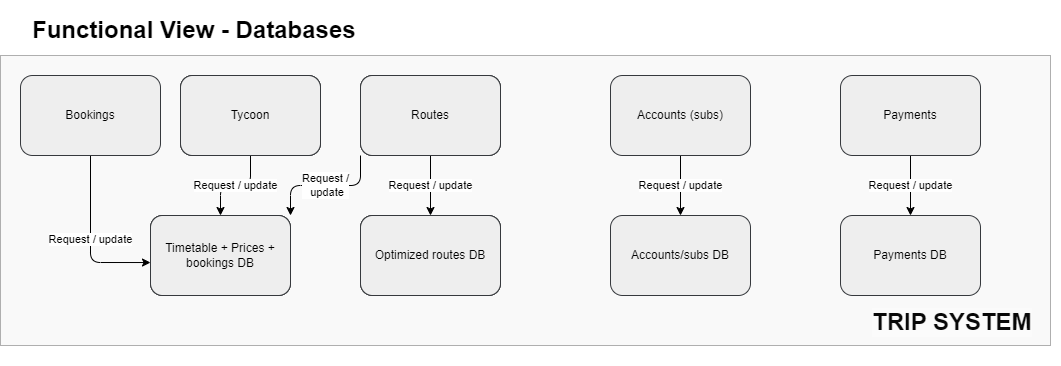
\includegraphics[width=\textwidth]{drawings/views_draft2/functional_view databases.png}
    \caption{Division of databases and their interaction with modules or stakeholders.}
    \label{fig:databases_view}
\end{figure}

\subsubsection*{Pros}
\begin{itemize}[noitemsep]
    \item \textbf{Enhanced Security} (Data Protection, Privacy): By segregating data across multiple databases, sensitive information is better protected, and access can be tightly controlled on a need-to-know basis.
    \item \textbf{Specialized Optimization} (Performance, Efficiency): Dedicated databases allow for optimization specific to their function, such as faster queries for timetable and booking data versus complex route optimization calculations.
\end{itemize}

\subsubsection*{Cons}
\begin{itemize}[noitemsep]
    \item \textbf{Increased Maintenance Overhead} (Maintainability, Complexity): Managing multiple databases adds complexity to the system's architecture, requiring more resources for maintenance and potentially higher costs.
    \item \textbf{Data Synchronization Challenges} (Reliability, Consistency): Ensuring data consistency across different databases can be challenging, especially in real-time, and may affect the system's overall reliability.
\end{itemize}

\subsection*{Option 2: Unified Centralized Database System}

This option proposes a centralized database architecture that consolidates all necessary information into a single, unified database system. It incorporates robust access control layers to manage data access based on module or user roles, ensuring that each part of the system accesses only the data it needs for operation. This model simplifies data management, enhances security through centralized control mechanisms, and facilitates easier updates and integrations. This model can be improved with having accounts database as a separate component, and keeping the rest of the databases central. In this way accounts data will be secure, and the rest of the systems will access accounts data anonymously via ids. Manage permissions for eacsh tycoon, on which info they can access (they shouldn't be able to connect name to bank account). In this way we can keep everything in the same place, but each tycoon api will have specificed access protocols. Tycoons can only update timetables and prices.

We can keep bookings data a DaaS, since it needs to be updated regularly and concurrently. The rest can be a server based database. Since we can cache routes we don't want cloud services for these. 

\subsubsection*{Pros}
\begin{itemize}[noitemsep]
    \item \textbf{Simplified Data Management} (Maintainability, Efficiency): Centralizing data storage simplifies the architecture by reducing the number of systems to manage, making it easier to maintain and update the database.
    \item \textbf{Improved Data Consistency} (Reliability, Integrity): A unified database ensures that all modules access the most current and consistent data, reducing the risk of discrepancies and errors.
    \item \textbf{Enhanced Integration Capability} (Scalability, Interoperability): With all data in one place, integrating new features, modules, or external systems becomes more straightforward, promoting scalability and interoperability.
\end{itemize}

\subsubsection*{Cons}
\begin{itemize}[noitemsep]
    \item \textbf{Risk of a Single Point of Failure} (Reliability, Availability): Centralizing data creates a single point of failure, which could potentially lead to system-wide outages affecting all functionalities if the database goes down.
    \item \textbf{Scalability Concerns} (Performance, Scalability): As the system grows, a centralized database might struggle with performance issues due to the increasing volume of data and concurrent access requests.
    \item \textbf{Complexity in Ensuring Data Protection} (Security, Privacy): Protecting a large, centralized repository of sensitive information poses significant challenges, requiring robust security measures to prevent unauthorized access and data breaches.
\end{itemize}

\subsection*{Option 3: Database per tycoon}

This option involves creating separate databases for each tycoon, allowing tailored data management and access controls specific to the needs and permissions of each tycoon. The aim is to provide a customized data storage solution that respects the autonomy and specific requirements of each railway tycoon, facilitating efficient and secure data handling.

\subsubsection*{Pros}
\begin{itemize}
    \item \textbf{Customization:} Each tycoon can have database features and structures tailored to their specific operational and data analysis needs, enhancing performance and usability.
    \item \textbf{Access Control:} Tycoon-specific databases simplify permission management, as each tycoon has access only to their relevant database, thereby automatically managing access permissions and minimizing the risk of unauthorized data access.
\end{itemize}

\subsubsection*{Cons}
\begin{itemize}
    \item \textbf{Management Overhead:} Maintaining separate databases for each tycoon increases the complexity of the system's architecture, requiring more resources for database management, synchronization, and ensuring consistency across databases.
    \item \textbf{Data Redundancy:} Shared data that is relevant to multiple tycoons, such as inter-tycoon route connections or passenger information, may need to be duplicated across databases, increasing storage requirements and complicating data synchronization.
\end{itemize}

This option was considered to provide high levels of customization and security by isolating each tycoon's data. However, it introduces significant challenges in terms of system complexity and data management efficiency. The requirement for tailored solutions for each tycoon, while beneficial for customization and security, potentially complicates the integration and consistent operation of the TrIP system as a whole.


\subsection*{Option 4: Hybrid cloud storage}
Less sensitive data can be stored in public cloud (timetables, and prices and bookings). Sensitive data (accounts, payments) gets stored in non-cloud databases, possibly one per tycoon, to avoid illegal data access.

\subsubsection*{Pros}
\begin{itemize}[noitemsep]
    \item \textbf{Tycoon specific access for accounts data} 
    \item \textbf{Secure and qucik access to data crucial data} 
    \item \textbf{Cheap storage for non-crucial data} 
\end{itemize}

\subsubsection*{Cons}
\begin{itemize}[noitemsep]
    \item \textbf{Can get expensive} 
    \item \textbf{Implementation of two different database types and their interactions setup}
\end{itemize}

\subsection*{Decision}

In adopting a hybrid cloud storage strategy (Option 4), we remain committed to the database-per-service pattern (Option 1), ensuring a modular and scalable system architecture. The majority of our data, including timetables, prices, and bookings, will be stored in public cloud services to benefit from their scalability and operational efficiency. Sensitive information, such as passenger and payment data, will be secured in private servers, maintaining strict adherence to security and compliance standards. This dual approach, combining the use of public cloud and private servers, aligns with our commitment to both security and efficiency. It also preserves the modularity and service-specific scalability afforded by the database-per-service pattern. Detailed deployment strategies and justifications are further elaborated in the deployment viewpoint documentation.
The goal is to achive high availability, which is crucial after Event 2, which requires less stringent maintainability and cost requirements. Maintainability and performance are increased by choosing database-per-service instead of a single database.

\subsection*{Consequences}

\textbf{Positive Consequences:}
\begin{itemize}
    \item Enhanced security for sensitive data by utilizing private servers, aligning with strict compliance and privacy standards.
    \item Improved scalability and operational efficiency for non-sensitive data through the use of public cloud services.
    \item Retained system modularity and ease of maintenance via the database-per-service pattern, facilitating targeted optimizations and updates.
\end{itemize}

\textbf{Negative Consequences:}
\begin{itemize}
    \item Potential complexity in managing a hybrid cloud environment, requiring robust synchronization and data management practices.
    \item Increased operational demands for ensuring seamless integration and security protocols between public cloud services and private servers.
\end{itemize}
\newpage
\subsection{Decision 6: Database technology}

\subsection*{Status}
Accepted. Reviewed after Event 4 (Data Leaks) with higher focus on security. 

\subsection*{Architectural Summary}
\begin{tabular}{|p{3.5cm}|p{10.5cm}|}
    \hline
    \textbf{In the context of} & Choosing appropriate database technology to store information about travels and payments, \\
    \hline
    \textbf{Facing} & The challenge of storing data coming from different tycoons systems in a cost-effective manner, \\
    \hline
    \textbf{To achieve} & Mainteinability, security, cost efficiency, performance and scalability \\
    \hline
    \textbf{We considered} & Option 1: SQL Database (e.g., PostgreSQL); Option 2: NoSQL Database (e.g., MongoDB); \\
    \hline
    \textbf{And decided for} & Option 1: SQL Database (e.g., PostgreSQL) \\
    \hline
    \textbf{Because} & It suits the kind of data we need to store, it is easier to source developers expertise and security is well tested, \\
    \hline
    \textbf{Accepting} & Potential difficulties in horizontal scaling, less flexibility in the data model. \\
    \hline
\end{tabular}

\subsection*{Concern}
The main staleholder's concerns related to this decision are the passengers request to have a good integration among different tycoons subscription, the TrIP owner request to keep maintenance costs low and the data protection required by government and passengers.

Related user stories are listed here:

\begin{itemize}[noitemsep]
    \item \userStoryEighteen,
    \item \userStoryTwentyNine,
    \item \userStoryThirty,
    \item \userStoryThirtyTwo,
\end{itemize}

\subsection*{Context}
In developing the TrIP system we are faced with the decision of choosing an appropriate database technology. This choice hinges on our need to ensure data integrity, support complex queries for transaction processing, and maintain scalability and security.
The database must handle a wide array of data, including user subscriptions, fare transactions, and station and route information, necessitating a robust system that supports complex queries and relational data structuring.
The architecture might include more than one databases, depending on the needs that will arise during later decisions.

\subsection*{Criteria}
\begin{itemize}[noitemsep]
    \item \textit{Cost efficiency} and \textit{mainteinability}.
    \item Comprehensive \textit{security} features to safeguard sensitive data.
    \item Data integrity and transactional consistency for financial transactions.
    \item Ability to support complex queries and relational data models.
    \item \textit{Scalability} to grow with the system's user base and data volume.
    \item \textit{Performance} under varying load conditions.
\end{itemize}

\subsection*{Option 1: SQL Database (e.g., PostgreSQL)}
A relational database model renowned for its strong consistency, ACID (Atomicity, Consistency, Isolation, and Durability) compliance, and the ability to efficiently handle complex queries and data relationships.
\begin{itemize}
    \item \textbf{Pro:} High data integrity and robust support for complex relational data structures.
    \item \textbf{Pro:} We have a highly structured data.
    \item \textbf{Pro:} More developers are familiar with it, more resources on the topic. It has a strong community and over 30 years of active development.
    \item \textbf{Pro:} Good with concurrency.
    \item \textbf{Pro:} Well tested security features like encryption, access control, SQL injection prevention, auditing capabilities.
    \item \textbf{Pro:} Open source and free.
    \item \textbf{Con:} Scalability challenges in horizontally distributed architectures compared to NoSQL options.
    \item \textbf{Con:} Requires accurate upfront planning of the data model due to its structured nature, thereby limiting flexibility.
\end{itemize}

\subsection*{Option 2: NoSQL Database (e.g., MongoDB)}
A distributed database system designed for scalability and flexibility, suitable for handling large volumes of diverse data types.
\begin{itemize}
    \item \textbf{Pro:} Offers superior scalability and flexibility for managing unstructured or semi-structured data.
    \item \textbf{Pro:} Enhances performance for non-structured data.
    \item \textbf{Con:} May compromise transactional integrity and consistency in favor of performance and scalability.
    \item \textbf{Con:} Relatively new, hence less well tested for security concerns.
\end{itemize}

\subsection*{Decision}
After thorough consideration, the decision is to implement an \textbf{SQL database}, specifically PostgreSQL for it being open source, for the TrIP system. This decision is underpinned by the SQL database's unmatched data integrity, support for complex transactions, and relational data modeling capabilities, which are crucial for the financial transactions and data relationships inherent in the TrIP system. Furthermore, train payment data are by nature very structured, don't give much creativity to the passengers, thus a relational database seems a more natural choice. Given the higher familiarity of developers, this choice addresses well the mainteinability required by the TrIP owner.

\subsection*{Consequences}
\textbf{Positive Consequences:}
\begin{itemize}
    \item Ensures high levels of data integrity and transactional consistency, critical for financial data and user subscriptions.
    \item Facilitates complex data queries and relationships, enabling sophisticated data analysis and reporting.
    \item Provides robust security features to protect sensitive data and comply with data protection regulations.
\end{itemize}
\textbf{Negative Consequences:}
\begin{itemize}
    \item May require additional strategies for scaling horizontally, such as implementing read replicas or sharding, to manage large data volumes and high traffic loads effectively.
    \item Could necessitate more intensive resource management and optimization to ensure performance at scale.
    \item A less flexible data model.
\end{itemize}
\newpage
\subsection{Decision 7: Customer Service}

\subsection*{Status}
Review.

\subsection*{Architectural Summary}
\begin{tabular}{|p{3.5cm}|p{10.5cm}|}
    \hline
    \textbf{In the context of} & Providing customer support to passengers, \\
    \hline
    \textbf{Facing} & The passengers' and customer service operators concern for quick information retrieval from the system, \\
    \hline
    \textbf{To achieve} & Timely and accurate, secure information retrieval and communication, \\
    \hline
    \textbf{We considered} & Option 1: Direct Access to Live Data; Option 2: Periodic Data Sync to a Dedicated Customer Service Database; Option 3: On-Demand Data Retrieval via Secure API; Option 4: Automated Reporting System\\
    \hline
    \textbf{And decided for} & Option 3: On-Demand Data Retrieval via Secure API \\
    \hline
    \textbf{Because} & It ensures security and good flexibility to integrate with changes in the customer service platform, \\
    \hline
    \textbf{Accepting} & Possible latency, an additional layer of complexity. \\
    \hline
\end{tabular}

\subsection*{Concern}
The primary concern is to ensure that customer service representatives have access to accurate and timely information to address passenger queries and resolve issues efficiently, without compromising data privacy.

\subsection*{Context}
This decision outlines the strategy for communication between the TrIP system and customer service teams to facilitate rapid and effective resolution of customer issues. Customer service teams require real-time access to passenger data, ticketing information, and system status to provide informed support. The chosen communication strategy must balance the need for information accessibility with system security and data privacy regulations.

\subsection*{Criteria}
\begin{itemize}
    \item Timeliness and accuracy of information communicated.
    \item Data privacy and security compliance.
    \item Ease of access for customer service representatives.
    \item Minimization of system complexity and maintenance.
    \item Integration with existing customer service platforms.
    \item Cost-effectiveness of the communication solution.
\end{itemize}

\subsection*{Option 1: Direct Access to Live Data}
Grant customer service representatives direct access to the live operational database with appropriate read-only permissions and privacy safeguards in place.
\subsubsection*{Pros}
\begin{itemize}
    \item Immediate access to data allows for quick customer service responses.
\end{itemize}
\subsubsection*{Cons}
\begin{itemize}
    \item Direct access to live data could pose security risks if not managed correctly.
\end{itemize}

\subsection*{Option 2: Periodic Data Sync to a Dedicated Customer Service Database}
Regularly synchronize relevant data from the operational database to a separate customer service database designed for query efficiency and tailored access control.
\subsubsection*{Pros}
\begin{itemize}
    \item Data syncing provides a stable environment tailored for customer service needs.
\end{itemize}
\subsubsection*{Cons}
\begin{itemize}
    \item Data syncing could lead to delays in information relay if not frequent enough.
\end{itemize}

\subsection*{Option 3: On-Demand Data Retrieval via Secure API}
Implement a secure API that allows customer service representatives to retrieve necessary data on-demand while maintaining strict access controls and audit trails.
\subsubsection*{Pros}
\begin{itemize}
    \item Secure API ensures data privacy and minimizes unnecessary data exposure.
\end{itemize}
\subsubsection*{Cons}
\begin{itemize}
    \item On-demand retrieval may introduce latency and requires robust API management.
\end{itemize}

\subsection*{Option 4: Automated Reporting System}
Develop an automated reporting system that provides customer service representatives with pre-defined reports and dashboards, reducing the need for direct data access.
\subsubsection*{Pros}
\begin{itemize}
    \item Automated reports streamline the information delivery process.
\end{itemize}
\subsubsection*{Cons}
\begin{itemize}
    \item Automated reporting may not cover all ad-hoc queries from customer service representatives.
\end{itemize}

\subsection*{Decision}
Option 3 is chosen: not enough requests to justify the burden of an additional database. Option 4 requires too much work from us. Option 1 doesn't seem secure enough.

\subsection*{Consequences}
\textbf{Positive Consequences:}
\begin{itemize}[noitemsep]
    \item \textbf{Security and Privacy:} The secure API maintains strict access controls and audit trails, enhancing the protection of sensitive passenger data and ensuring compliance with data privacy regulations.
    \item \textbf{Flexibility:} Allows for flexible, on-demand data retrieval, which can be easily adapted or expanded to meet evolving requirements, providing a scalable solution for future needs.
    \item \textbf{Integration Capabilities:} Facilitates easier integration with existing or future customer service platforms, making the option highly scalable and versatile for a range of services.
\end{itemize}

\textbf{Negative Consequences:}
\begin{itemize}[noitemsep]
    \item \textbf{Latency and Performance:} The on-demand nature of data retrieval may introduce latency, requiring robust API management and performance optimization to ensure timely customer service responses.
    \item \textbf{Complexity in API Management:} Managing the API adds a layer of complexity, including version control, access management, and security updates, which necessitates dedicated resources.
    \item \textbf{Dependence on External Systems:} Reliance on external services or platforms for the API functionality can pose risks related to their availability and performance, necessitating contingency planning for high availability and redundancy.
\end{itemize}
\newpage
\subsection{Decision 8: Interaction with ticket scanners}

\subsection*{Status}
Open
\subsection*{Architectural Summary}


\subsection*{Concern}
Passengers want a seamless travel experience, without being mistakenly blocked at the turnstiles.
Tycoons want to admit only paying passengers in trains, avoiding controllers costs.
Turnstiles need to communicate with the system to ensure correct and quick verification of the requisites to be allowed in the station.

\subsubsection*{User Stories}
The decision on how turnstiles interact with the payment system is integral to ensuring a seamless travel experience and securing access to train areas. Below, we detail specific user stories connected to this architectural decision, highlighting the requirements and expectations from various stakeholders.

\begin{enumerate}[noitemsep]
    \item \textbf{User Story 1 (Frequent Traveler's Monthly Pass)}: A comprehensive monthly pass needs to be recognized by the turnstiles, necessitating a system that supports seamless access for subscribers.
    
    \item \textbf{User Story 2 (Online Balance Check for Multi-Network Travel Card)}: The system requires turnstiles to accurately read and verify travel card balances to prevent entry issues, emphasizing the need for an integrated payment system.
    
    \item \textbf{User Story 15 (Prevention of Payment for Temporarily Blocked Routes)}: This story underscores the importance of turnstiles having up-to-date information on route availability to avoid mistakenly blocking passengers.
    
    \item \textbf{User Story 16 (Single Ticket for All Train Networks)}: Turnstiles must effectively communicate with the payment system to recognize and approve tickets valid across different networks, ensuring seamless travel.
    
    \item \textbf{User Story 26 (Real-time Updates for Station Managers)}: The technology supporting real-time updates can also enhance turnstile interactions, ensuring entry permissions reflect current ticketing information based on schedules and disruptions.
    
    \item \textbf{User Story 27 (Integration with Maintenance Scheduling)}: Turnstiles must adapt to maintenance schedules, allowing for adjustments in access permissions, which suggests the need for a flexible and responsive payment system.
    
    \item \textbf{User Story 23 (Payment System Integration for Tycoons)}: The story relates to the seamless integration of turnstiles with updated payment systems, crucial for maintaining high service levels and secure access.
\end{enumerate}

These user stories collectively highlight the diverse requirements for the turnstile and payment system interaction, from seamless access and real-time information integration to flexibility in handling various ticketing formats and system updates.
The problem can be made more abstract, as the interaction with the turnstile can be similar to the following interactions:
\begin{itemize}
    \item interaction with a controller who scans the ticket or any proof of subscription.
    \item interaction with a scanner onboard a bus.
\end{itemize}

\subsection*{Context}

Most stations, expecially the big ones, have turnstiles to avoid people without tickets to enter the trains area.
The turnstiles should communicate with the system to ensure this. A decision should be taken on who to admit in the station.
This logic could be provided by the station manager or by the tycoons, or even by TrIP managment.
How do the passenger input its ticket or subscription or prepaid card to the turnstile?
How does the turnstile communicate with the system to verify if the passenger has the right to enter the station?

\subsection*{Criteria}
\begin{itemize}
    \item Allow passengers to scan tickets or multiplatform travel cards (if they exists) at turnstiles.
    \item Don't allow people without the appropriate tickets or subscriptions or cards.
    \item Possibly allow people to scan when they enter and when they exit and calculate a fare (this might depend on agreements between tycoons). 
    \item Possibly communicate station usage data to the system.
    \item Possibly allow credit/debit card scan.
    \item Allow balance check for charged cards.
\end{itemize}

\subsection*{Option 1: Add a ticket checker and a user state modules to authorize passengers}
After scanning a ticket or badge, the user state should be updated, in order to calculate the fare price for fillable card holders or for the scanning of bank cards (debit credit).
The ticket or badge should be checked by the single ticket checker module or by the account management to insure consistency.
In case of the scanning of bank cards, the user state module needs to communicate with payment management, in order to proceed with the actual payment.
The scanning of bank cards and fillable cards create the needs for a calculation of appropriate revenue share between different tycoon. This should be the topic of a future decision or might be incorporated in this one.
\begin{figure}[ht]
    \centering
    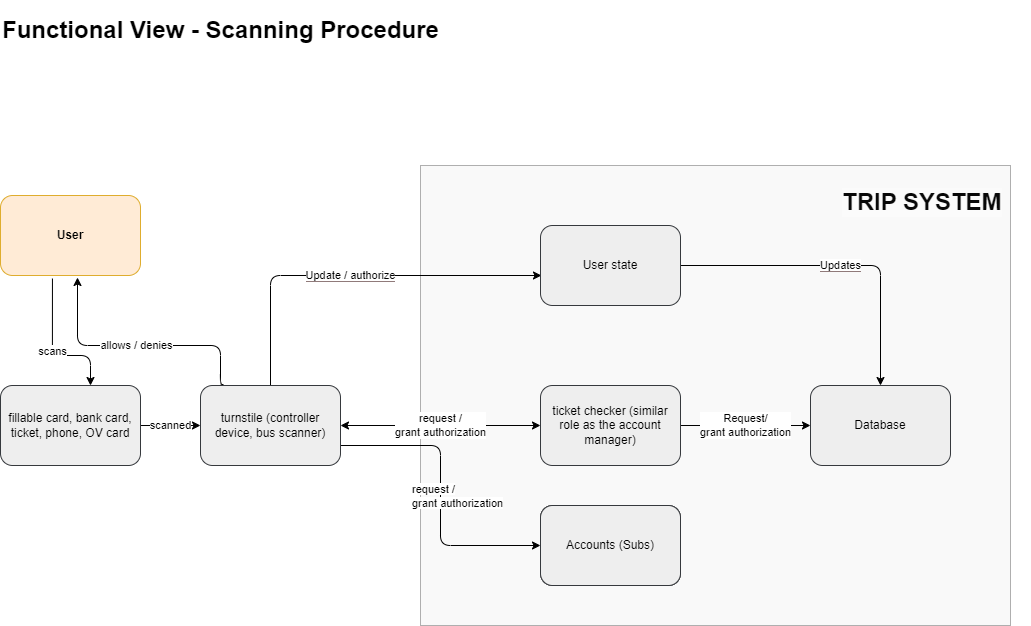
\includegraphics[width=\textwidth]{drawings/views_draft2/functional_view turnstiles.png}
    \caption{Interaction with a ticket scanner.}
    \label{fig:ticket_scanner}
\end{figure}

\subsection*{Option 2: Allow fillable cards, account cards and tickets, not bank cards}
Not allowing bank cards at turnstiles simplifies the job of turnstiles.
Also, how can a controller check if the traveller have scanned a bank card when entering the turnstile?
We can have the turnstile print a ticket with a barcode or QR code.


\subsection*{Decision}

\subsection*{Consequences}
\textbf{Positive Consequences:}
% \begin{itemize}
% \end{itemize}
\textbf{Negative Consequences:}
% \begin{itemize}
% \end{itemize}
\newpage
\subsection{Decision 9: Account management and authentication}

\subsection*{Status}
Review

\subsection*{Architectural Summary}
\begin{tabular}{|p{3.5cm}|p{10.5cm}|}
    \hline
    \textbf{In the context of} & letting passengers authenticate to their accounts to handle subscriptions, \\
    \hline
    \textbf{Facing} & the passengers' concern for user-friendlyness and the tycoon request for integration between their subscriptions systems, also ensuring sensitive data privacy, \\
    \hline
    \textbf{To achieve} & security, usability and integrabiliy, \\
    \hline
    \textbf{We considered} & Option 1: Anonymous card; Option 2: Bank credit card; Option 3: Phone app; Option 4: Nominal card; Option 5: NFC reader/Google Wallet\\
    \hline
    \textbf{And decided for} & a hybrid approach where multiple authentication methods are allowed, both nominal (like a dedicated card) and anomymous (like a fillable card);\\
    \hline
    \textbf{Because} & it ensures high usability for many kinds of passengers, only two readers are needed (NFC and QR) at turnstiles, which keeps costs controlled, security is ensured by tokenization, \\
    \hline
    \textbf{Accepting} & Higer system complexity, more complicated development and maintenance. \\
    \hline
\end{tabular}

\subsection*{Concern}
Ensuring a secure, user-friendly, and efficient process for account creation, management, and authentication for a variety of users, while maintaining data privacy and system integrity.

\subsection*{Context}
The TrIP system requires a flexible and secure method for user authentication that accommodates various levels of user interaction and convenience. The chosen solution must integrate seamlessly with the existing ticketing and payment infrastructure and support a range of devices and technologies used by passengers.

\subsection*{Criteria}
\begin{itemize}
    \item Secure storage and handling of personal and financial data.
    \item Ease of account creation and management for passengers.
    \item Seamless integration with existing turnstile and payment systems.
    \item Flexibility to support different methods of authentication, including cards and digital wallets.
    \item High availability and reliability of the authentication system.
\end{itemize}

\subsection*{Option 1: Anonymous card}
\begin{itemize}
    \item \textbf{Pro:} Ensures passenger privacy and quick adoption for casual users.
    \item \textbf{Con:} Limited capabilities for account management and tracking passenger history.
\end{itemize}

\subsection*{Option 2: Bank credit card}
\begin{itemize}
    \item \textbf{Pro:} Streamlines payment process by integrating with existing financial systems.
    \item \textbf{Con:} Relies on external systems, which may pose integration challenges and dependency risks.
\end{itemize}

\subsection*{Option 3: Phone app}
\begin{itemize}
    \item \textbf{Pro:} Provides a versatile platform for account management, payments, and ticket validation via QR codes or NFC.
    \item \textbf{Con:} Requires smartphone access, possibly excluding certain passengers demographics.
\end{itemize}

\subsection*{Option 4: Nominal card}
\begin{itemize}
    \item \textbf{Pro:} Offers a physical, personalized token for account access and ticket validation.
    \item \textbf{Con:} May introduce additional costs for production and distribution of cards.
\end{itemize}

\subsection*{Option 5: NFC reader/Google Wallet}
\begin{itemize}
    \item \textbf{Pro:} Leverages existing NFC technology in smartphones for easy tap-and-go access at turnstiles.
    \item \textbf{Con:} Implementation cost and required NFC-capable turnstiles may be high.
\end{itemize}

\subsection*{Decision}
The decision is to implement a hybrid approach, integrating a phone app (with NFC capabilities and linked to bank accounts) for regular users, along with an anonymous fillable card for tourists and a physical nominal card for those who prefer or require a physical token. The hybrid approach balances convenience with coverage for all passenger types.
A tokenization service can be implied, so that no sensitive data is stored, but only tokens representing it, which transfer the security risk and the compliance requirements to specialized companies.

\subsection*{Consequences}
\textbf{Positive Consequences:}
\begin{itemize}
    \item Provides a comprehensive solution covering the needs of various passenger groups, increasing system accessibility and passenger satisfaction.
    \item Enhances security by offering multiple authentication methods, each with its own set of security protocols.
    \item Encourages digital transformation and supports a move towards a more contactless, efficient user experience.
\end{itemize}
\textbf{Negative Consequences:}
\begin{itemize}
    \item May increase complexity and cost of the system, both in development and maintenance.
    \item The need to support multiple authentication methods can complicate infrastructure and operational processes.
    \item Potential resistance from passengers who are less technologically adept or prefer traditional methods.
\end{itemize}
This decision supports the TRIP system's objective to provide a secure, convenient, and inclusive environment for all types of passengers while recognizing the need to manage operational and development complexities.

\newpage
\subsection{Decision 10: Data update from tycoons or station management}

\subsection*{Status}
Accepted.
\subsection*{Architectural Summary}
\begin{tabular}{|p{3.5cm}|p{10.5cm}|}
    \hline
    \textbf{In the context of} & allowing data update (like timetables and fare prices) from tycoons, \\
    \hline
    \textbf{Facing} & the need to quickly allow addition of new tycoons, fair competition between tycoons, passengers' request of correct information; \\
    \hline
    \textbf{To achieve} & tycoons' usability, reliability for passengers, \\
    \hline
    \textbf{We considered} & Option 1: Tycoon API for interactions with databases; Option 2: Real time information requests to tycoon systems and tycoon-specific API \\
    \hline
    \textbf{And decided for} & Option 1: Tycoon API for interactions with databases;\\
    \hline
    \textbf{Because} & Convers Event 1 specifically, ensures data consistency across tycoons-specific timetables/price, improves mainteinability of the system, \\
    \hline
    \textbf{Accepting} & Potential resistance from some tycoons, API management, data management overhead. \\
    \hline
\end{tabular}


\subsection*{Concern}
The system needs to receive information and updates from the tycoons. 
This can be for instance:
\begin{itemize}
    \item train or buses time tables;
    \item static data like stations ownership and connections (static meaning that it changes less often than other information);
    \item last-minute updates like disruptions, delays, interruptions.
\end{itemize}
The information above are necessary for the following quality attributes:
\begin{itemize}
    \item \textit{reliability} of the system required by the tycoons (priority 2), as passengers needs to always be able to pay for their travels (hence updated timetables are important);
    \item \textit{usability} of the system for the passengers (priority 2), who wants as few actions on their own initiative as possible;
\end{itemize}

The system also need to give acces to some information to the tycoon, with proper care to not expose information from other tycoons:
\begin{itemize}
    \item payment received by subscribers;
    \item bought tickets;
    \item booking information;
    \item data from the turnstiles scanners. 
\end{itemize}

Scalability here is an important concern, as this data needs to be provided, requested and stored by the system for different tycoons.
After Event 1, the priority for \textit{Scalability} has been set to two, so the system needs to be flexible enough to easily access new tycoons also from different kind of transport.

Also \textit{security} and \textit{privacy} here are paramount, as only the strictly necessary and allowed information can be exposed.

\subsubsection*{User stories}

\subsection*{Context}
The systems keeps data stored on multiple databases. 
Some of them needs to give some degree of access to the tycoons and the customer service of the TrIP system:
\begin{itemize}
    \item Tickets database;
    \item Payments database;
    \item Accounts and subscriptions database;
\end{itemize}

Others needs to let the tycoon feed them, such as the Timetable databases, which holds information about train schedules,
prices and bookings.

\subsubsection*{QA Scenario} % not always needed I believe
Consider the scenario of adding/removing a tycoon, adding/removing routes and stations.
\subsection*{Criteria}
\begin{itemize}
    \item Data correctness in the system, expecially after event 2.
    \item Ease of use from the tycoons to update the system and get data for analytics.
    \item Performance and availability: data should flow into the system with reasonable speed.
    \item Adding new tycoons should be easy.
\end{itemize}

\subsection*{Option 1: Tycoon API for interactions with databases}

We can add a layer between the TrIP system and the Tycoons, as an API which gives a set of querying rights to tycoons to export the data they need and forces them a format of data to be provided.

Forcing tycoons to a certain format is possible because both bus and train system can be abstracted to a graph, where nodes are stations and edges are connections.
They both have times for connections and prices to submit, together with bookings availabilities.
\subsubsection*{Pros}
\begin{itemize}[noitemsep]
    \item \textbf{Scalability}: by forcing a format of queries and data submission, we abstract away from the specifics of a way tycoons provide their connection services.
    \item \textbf{Maintainability}: we let our system have its own independent and unique data representation, ensuring a common data format.
    \item \textbf{Performance}: Routes optimization can be precompute with timetables and only updated when new information come from the tycoond.
\end{itemize}
\subsubsection*{Cons}
\begin{itemize}[noitemsep]
    \item \textbf{Usability} for the tycoon: Interfacing with an API needs some work from the tycoons IT department, to ensure the TrIP system is properly updated.
    \item \textbf{Operational cost}: storing lots of information on the TrIP system requires the management of multiple databases.
\end{itemize}


\subsection*{Option 2: Real time information requests to tycoon systems and tycoon-specific API}
Also asking data from tycoons periodically from the system is a possibility. In this case the TrIP system is
responsible for the data querying and feeding, thus it should be able to interact with each tycoon system with a specific API.
\subsubsection*{Pros}
\begin{itemize}[noitemsep]
    \item \textbf{Usability}: The system can provide almost real-time to users, only limited by the technical capabilities of tycoons systems.
    \item \textbf{Operational costs}: The system doesn't need to store as much information, as it can pass it to the tycoons, let them store it and then cancel it.
\end{itemize}
\subsubsection*{Cons}
\begin{itemize}[noitemsep]
    \item \textbf{Maintainability} and \textbf{Scalability}: This requre a lot of implementation every time a new tycoon enters.
\end{itemize}

\subsection*{Decision}
As the importance of scalability has been increased by event 1, Option 1 seems the most natural.
Furthermore, operational cost has reduced importance after event 2, which limits the cons of option 1.
It ensures high integrability of the system with the tycoons and customer services systems.
Also availability can be improved with option 1, as we cannot ensure high availability of tycoon system, while we can deploy tactics to ensure our own databases availabiliy. The specific choice of tactics will be outlined in the deployment view.

\subsection*{Consequences}
\textbf{Positive Consequences:}
\begin{itemize}
    \item Adding new tycoons would be easy for the TrIP system.
    \item Standardized data is exchanged and managed.
    \item Load management efficiency: the TrIP system is responsible for its own load management, instead of relying on tycoons systems.
    \item High accuracy of data thanks to standardization.
    \item Tycoons can potentially share analytical tools, having all the same interface.
    \item API acts as a gatekeeper, to keep tycoons from accessing to unwanted information. This should be reflected on future decisions meant at defining specific tactics.
\end{itemize}
\textbf{Negative Consequences:}
\begin{itemize}
    \item Potential resistance from some tycoons (we could mitigate by providing technical support);
    \item API stability: updates to our API might require changes from many tycoons, therefore the API will be by definition difficult to modify. Also here a proper technical support could be provided to mitigate the issue.
    \item Data management overhead: we need data storage and backup and security concerns. Storing payment data can be done in an anonymized way using tokenization services.
\end{itemize}
\newpage
\subsection{Decision 11: Disruptions and Route Updates}

\subsection*{Status}
Open

\subsection*{Architectural Summary}

\begin{tabular}{|p{3.5cm}|p{10.5cm}|}
    \hline
    \textbf{In the context of} & Managing disruptions effectively within the TrIP system. \\
    \hline
    \textbf{Facing} & The need to minimize inconvenience for passengers during disruptions. \\
    \hline
    \textbf{To achieve} & A balance between rapid response and clear communication with passengers. \\
    \hline
    \textbf{We considered} & \begin{tabular}{@{}l@{}}1. Real-Time Alert System, \\ 2. Manual Intervention Protocol, \\ 3. Threshold-Based Re-Optimization, \\ 4. Continuous Optimization.\end{tabular} \\
    \hline
    \textbf{And decided for} & Option 3: Threshold-Based Re-Optimization. \\
    \hline
    \textbf{Because} & It optimally balances operational efficiency and passenger communication, focusing resources on significant disruptions. \\
    \hline
    \textbf{Accepting} & The potential oversight of minor delays and the reliance on terminal-based information. \\
    \hline
\end{tabular}


\subsection*{Concern}
The main concern is to ensure minimal inconvenience to passengers during train disruptions while maintaining transparent communication and providing alternative solutions.

Related user stories are listed below:
\begin{itemize}
    \item \textbf{User Story 26:} As a station manager, I want the system to offer real-time updates on train schedules and network disruptions so that I can keep passengers informed and manage station flow effectively.
\end{itemize}

\subsection*{Context}
Train disruptions can occur due to various reasons such as maintenance issues, accidents, or natural events. The system needs to be able to quickly respond to such incidents, inform affected passengers, and offer alternatives to ensure continued service.
This is important for our system as a consequence of the choice to handle route optimization within the system.

\subsection*{Criteria}
\begin{itemize}
    \item Rapid detection and response to disruptions.
    \item Clear and timely communication with passengers.
    \item Provision of alternative transport options.
    \item Integration with existing operational and communication systems.
    \item Minimization of negative impact on passenger experience.
    \item Compliance with safety and regulatory standards.
\end{itemize}


\subsection*{Option 1: Real-Time Alert System}
\subsubsection*{Pros}
\begin{itemize}
    \item Quickly informs passengers about disruptions.
\end{itemize}
\subsubsection*{Cons}
\begin{itemize}
    \item Requires passengers to actively seek updates.
\end{itemize}

\subsection*{Option 2: Manual Intervention Protocol}
\subsubsection*{Pros}
\begin{itemize}
    \item Personalized assistance to passengers for rebooking and advice.
\end{itemize}
\subsubsection*{Cons}
\begin{itemize}
    \item Complex to implement and integrate with existing systems.
\end{itemize}

\subsection*{Option 3: Threshold-Based Re-Optimization}
\subsubsection*{Pros}
\begin{itemize}
    \item Focuses on significant disruptions, optimizing system and passenger resources.
    \item Reduces the number of unnecessary passenger notifications for minor issues.
\end{itemize}
\subsubsection*{Cons}
\begin{itemize}
    \item Minor delays may not trigger system responses, potentially accumulating unnoticed.
    \item Terminal-based information may not effectively reach all passengers.
\end{itemize}

\subsection*{Option 4: Continuous Optimization}
\subsubsection*{Pros}
\begin{itemize}
    \item Offers constant adaptability to real-time conditions, potentially enhancing system responsiveness.
\end{itemize}
\subsubsection*{Cons}
\begin{itemize}
    \item Could result in frequent, possibly confusing updates for passengers.
    \item May demand significant computational resources, affecting system efficiency.
\end{itemize}


\subsection*{Decision}
We choose Option 3: Threshold-Based Re-Optimization for its strategic focus on significant disruptions. This decision is made recognizing that while minor disruptions may be overlooked, the emphasis on substantial delays aligns with our goal of efficiently managing resources and maintaining a high-quality passenger experience.

\subsection*{Positive Consequences}
\begin{itemize}
    \item Efficient resource allocation by focusing on significant disruptions ensures the system's responsiveness to passenger needs during major incidents.
    \item Reduction in passenger notification fatigue by limiting communications to significant events, thereby enhancing the relevance and impact of messages received.
    \item Improved system performance and cost efficiency by avoiding unnecessary re-optimization processes for minor disruptions.
\end{itemize}

\subsection*{Negative Consequences}
\begin{itemize}
    \item Potential for minor disruptions to accumulate and impact passenger experience if they are not addressed due to falling below the set threshold.
    \item Risk of insufficient communication if passengers are not near terminals and thus may miss critical information about disruptions and re-optimizations.
    \item Challenges in setting an appropriate threshold that accurately distinguishes between minor and significant disruptions, requiring continuous evaluation and adjustment.
\end{itemize}

\newpage
\subsection{Decision 12: Serverless vs. Servers for Calculations}

\subsection*{Status}
Open

\subsection*{Architectural Summary}
\begin{tabular}{|p{3.5cm}|p{10.5cm}|}
    \hline
    \textbf{In the context of} & choosing to deploy TRiP system on cloud or on physical servers, \\
    \hline
    \textbf{Facing} & cost-effectiveness required by the TRiP owner, scalability and performance needs, \\
    \hline
    \textbf{To achieve} & high availability of the system together with security of passengers data, \\
    \hline
    \textbf{We considered} & Option 1: Serverless architecture; Option 2: Dedicated Servers; Option 3: Hybrid Approach\\
    \hline
    \textbf{And decided for} & Option 3: Hybrid Approach \\
    \hline
    \textbf{Because} & it ensures security where it is needed and cost-effectiveness for the rest of the system, \\
    \hline
    \textbf{Accepting} & Higer operation costs and more involved initial setup and mainentance. \\
    \hline
\end{tabular}

\subsection*{Concern}
The primary concern is to select a computational architecture that balances scalability, cost, performance, and data privacy for processing passenger data and transactional information.

\subsection*{Context}
The computational backbone of the TrIP system must handle variable workloads efficiently, especially during peak hours when route calculations and payment processing are at their highest demand. Additionally, the system must maintain data privacy and adhere to regulatory compliance.

\subsection*{Criteria}
\begin{itemize}
    \item Scalability to handle peak and off-peak loads.
    \item Cost-effectiveness, including operational and maintenance costs.
    \item Performance in terms of latency and throughput.
    \item Data privacy and control.
    \item Compliance with data protection and privacy laws.
    \item Ease of maintenance and updates.
\end{itemize}

\subsection*{Option 1: Serverless architecture}
Adopting a serverless architecture where the service provider dynamically manages the allocation of machine resources.
\subsubsection*{Pros}
\begin{itemize}
    \item Cost efficiency during low usage.
    \item No need for server maintenance.
    \item Automatic scaling.
\end{itemize}
\subsubsection*{Cons}
\begin{itemize}
    \item Potential for increased latency.
    \item Less control over data.
    \item Possible security concerns.
\end{itemize}

\subsection*{Option 2: Dedicated Servers}
Using dedicated servers, either on-premises or hosted, to handle all computations.
\subsubsection*{Pros}
\begin{itemize}
    \item Greater control over data.
    \item Potentially better performance.
    \item Consistent availability.
\end{itemize}
\subsubsection*{Cons}
\begin{itemize}
    \item Higher upfront costs.
    \item Requires dedicated IT staff for maintenance.
    \item Might be underutilized during off-peak times.
\end{itemize}

\subsection*{Option 3: Hybrid Approach}
Implementing a hybrid system that uses a combination of serverless architecture for less sensitive and highly variable workloads, and dedicated servers for more predictable workloads and data-intensive tasks requiring stringent privacy controls.
\subsubsection*{Pros}
\begin{itemize}
    \item Balances the benefits of both serverless and dedicated servers.
    \item Provides scalability while maintaining data privacy for sensitive operations.
\end{itemize}
\subsubsection*{Cons}
\begin{itemize}
    \item Increased complexity in managing two different environments.
    \item Potential for higher operational costs.
\end{itemize}

\subsection*{Decision}
As the focus on security have increased after Event 4 and the TRiP owner is more prone on spending, we pick option 3. This way, all the privacy-critical operations and data storages will be done in private clouds, while operations and storages of public data (such as the timetables),
will be on public data, guaranteeing cost-effectiveness and less maintenance concerns.
We choose to store and operate with accounts in the system identifying them via an account ID. The mapping between this account IDs and the account private information (such as name, contacts, etc.) should be stored in a in-house private server.
Communication with this database need to be encrypted to guarantee compliance with GDPR, write access to it can only be done by passengers while managing their accounts and read writes can be guaranteed only to officials verifying tickets onboard trains.
Note that credit card data are stored in the system as tockens, so they are not considered sensitive information.

\subsection*{Consequences}
\textbf{Positive Consequences:}
\begin{itemize}
    \item \textbf{Scalability:} Efficient adaptation to variable workloads with serverless, and reliable performance for constant workloads on dedicated servers.
    \item \textbf{Cost-Effectiveness:} Reduced operational costs through serverless computing for dynamic workloads.
    \item \textbf{Performance:} Optimized performance for data-intensive tasks on dedicated servers.
    \item \textbf{Security and Data Privacy:} Enhanced control over sensitive data processing and storage.
\end{itemize}

\textbf{Negative Consequences:}
\begin{itemize}
    \item \textbf{Complexity:} Increased management complexity blending serverless and server environments.
    \item \textbf{Operational Costs:} Potential rise in costs associated with maintaining dedicated server infrastructure.
    \item \textbf{Integration Challenges:} Difficulties in seamless operation between serverless and server-based components.
    \item \textbf{Dependency on Cloud Providers:} Reliance on third-party services for serverless components.
\end{itemize}

\newpage
\subsection{Decision 13: Revenue Division Strategies}

\subsection*{Status}
To be decided.

\subsection*{Architectural Summary}
\begin{tabular}{|p{3.5cm}|p{10.5cm}|}
    \hline
    \textbf{In the context of} & Developing a fair and transparent revenue division strategy among the tycoons within the TRiP system. \\
    \hline
    \textbf{Facing} & The challenge of equitably distributing revenue that accurately reflects each tycoon's contribution to the network. \\
    \hline
    \textbf{To achieve} & A revenue division model that is accepted by all stakeholders and supports the system's long-term sustainability. \\
    \hline
    \textbf{We considered} & Tap Cards Onboard Transport Vehicles, Annual Value-Based Share, Negotiated Shares. \\
    \hline
    \textbf{And decided for} & We advise for Option 1: Tap Cards Onboard Transport Vehicles. \\
    \hline
    \textbf{Because} & It offers a direct link between revenue and service usage, encouraging improvements in service quality and ridership. \\
    \hline
    \textbf{Accepting} & This is fundamentally a business decision that the TRiP board should make. We can accommodate the chosen strategy accordingly. \\
    \hline
\end{tabular}

\subsection*{Concern}
The main concern of the users in the context of this decision are descibed by the following user stories: 
\begin{itemize}
    \item User Story 21: Tycoons require accurate revenue tracking.
    \item User Story 23: Tycoons demand minimal disruption to existing infrastructure.
    \item User Story 24: Tycoons need analytics and insights for business decisions.
\end{itemize}

\subsection*{Context}
The revenue division strategy impacts the following functional elements and databases within the Train Inter Payment System (TrIP):
\begin{itemize}
    \item Payment Terminals: Interface for collecting revenue data.
    \item Tycoon-Specific Systems: Must integrate with revenue distribution logic.
    \item Databases:
    \begin{itemize}
        \item Ticket Database: Stores ticket sales data.
        \item Payment Database: Tracks completed transactions.
        \item Accounts and Subscriptions Database: Manages passenger subscriptions impacting revenue sharing.
    \end{itemize}
    \item Booking Management Module: Influences revenue calculation based on booked seats.
    \item Account and Subscription Management Module: Central to managing subscription-related revenue data.
\end{itemize}

\subsection*{Criteria}
The goal of this decision is to satisfy the user's concerns while safeguarding the other quality attribute requirements of the system. The main QAs affected by this decision are listed here:
\begin{itemize}
    \item Functional Suitability: Functionally complete, correct, and appropriate method for revenue distribution.
    \item Performance Efficiency: Strategy must not adversely affect system response times or resource utilization.
    \item Compatibility: Must coexist and interoperate with the tycoons' diverse systems and databases.
    \item Security: Ensuring confidentiality and integrity of revenue data.
    \item Maintainability: Ability to analyze, modify, and test revenue division logic as needed.
    \item Reliability: Fault tolerance and availability of the revenue division process.
    \item Flexibility: Adaptability and scalability of the strategy to accommodate new tycoons or changing business models.
\end{itemize}

\subsection*{Option 1: Tap Cards Onboard Transport Vehicles}
Allocate revenue to the tycoon operating each transport vehicles based on passenger tap card data. This approach directly links revenue to individual train usage.
\begin{itemize}
    \item \textit{Pros}: Directly correlates revenue with service usage, incentivizing tycoons to improve service quality and increase ridership.
    \item \textit{Cons}: May not fully account for the value of network-wide contributions, such as infrastructure maintenance or off-peak services.
\end{itemize}
    
\subsection*{Option 2: Annual Value-Based Share}
Distribute revenue based on a combination of the value of each tycoon's contributions (infrastructure and services) and ticket sales data from the previous year.
\begin{itemize}
    \item \textit{Pros}: Acknowledges both the operational and capital contributions of tycoons, potentially offering a more balanced revenue share.
    \item \textit{Cons}: Risks disadvantaging new entrants or those expanding services, as it relies on historical data.
\end{itemize}

\subsection*{Option 3: Negotiated Shares}
Tycoons negotiate revenue shares periodically, based on a set of agreed criteria (e.g., service quality, passenger numbers, network investment).
\begin{itemize}
    \item \textit{Pros}: Allows for flexibility and adaptability in revenue sharing, can directly address the specific contributions and needs of each tycoon.
    \item \textit{Cons}: Could lead to conflicts or prolonged negotiations, potentially destabilizing the revenue sharing process.
\end{itemize}

\subsection*{Decision}
While we advise for Option 1: Tap Cards Onboard Transport Vehicles for its direct correlation between revenue and service usage, we recognize that the final decision rests with the TRiP board. This decision is seen as strategic and will significantly impact the partnership dynamic among the tycoons. As such, we emphasize that this choice should be made at the business level, and we are prepared to support and implement the board's decision to best serve the system's objectives and stakeholder needs.

\subsection*{Consequences}
\textbf{Positive Consequences:}
\begin{itemize}
    \item Enhances transparency and fairness in revenue sharing, directly linking earnings to each tycoon's service usage.
    \item Incentivizes tycoons to focus on improving service quality and expanding ridership.
    \item Adaptable to system expansions and the introduction of new services or tycoons.
\end{itemize}
\textbf{Negative Consequences:}
\begin{itemize}
    \item Potential challenges in accurately tracking and attributing revenue, especially in mixed-use or multi-leg journeys.
    \item May require significant infrastructure investment for full implementation.
    \item Could lead to disputes over revenue attribution and require continuous oversight and adjustment.
\end{itemize}

\newpage
\subsection{Decision 14: Handling Network Outages}

\subsection*{Status}
Open


\subsection*{Architectural Summary}
\begin{tabular}{|p{3.5cm}|p{10.5cm}|}
    \hline
    \textbf{In the context of} &  \\
    \hline
    \textbf{Facing} &  \\
    \hline
    \textbf{To achieve} & \\
    \hline
    \textbf{We considered} & \\
    \hline
    \textbf{And decided for} & \\
    \hline
    \textbf{Because} &  \\
    \hline
    \textbf{Accepting} &  \\
    \hline
\end{tabular}

\subsection*{Concern}
Ensuring system resilience and continuous operation during network disruptions.
\subsubsection*{User Stories}
\begin{itemize}
    \item Users expect ticket validation to work even during network outages.
    \item Tycoons require the system to handle transactions securely and efficiently, irrespective of network status.
\end{itemize}

\subsection*{Context}
Network outages pose significant challenges to real-time processing capabilities, affecting ticket validations and financial transactions.

\subsection*{Criteria}
\begin{itemize}
    \item Minimize service disruption during network outages.
    \item Ensure data security and integrity, especially for financial transactions.
    \item Optimize local data storage to balance operational continuity with security risks.
\end{itemize}

\subsection*{Option 1: Delayed Processing}
Transactions are processed once network connectivity is restored, minimizing the need for local data storage but risking transaction backlog.

\subsection*{Option 2: Local Caching}
Local caching of critical data to enable processing during outages, with careful consideration of security implications due to increased local data storage.

\subsection*{Decision}
A combination of Option 1 and strategic caching for essential data will be used for delayed processing. This approach is chosen to maintain service reliability while addressing security concerns.
This decision balances the need for uninterrupted service during network outages against the risks associated with local data storage. It considers the priority of user experience and security as per stakeholder requirements and aligns with previous decisions to enhance system resilience.

\subsection*{Consequences}
\textbf{Positive Consequences:}
\begin{itemize}
    \item Maintains ticket validation and system operations during network outages, enhancing user experience.
    \item Reduces the risk of service disruption, aligning with the expectations of users and tycoons.
    \item Balances operational needs with security concerns through selective data caching.
\end{itemize}
\textbf{Negative Consequences:}
\begin{itemize}
    \item May introduce a risk of negative balances due to delayed processing of financial transactions.
    \item Increases system complexity with the need to manage both delayed processing and data caching mechanisms.
    \item Poses potential security risks related to the local storage of sensitive data, despite limited caching.
\end{itemize}

\newpage
\section{Context Viewpoint}

\subsection{View: Stakeholders}

\subsubsection{Model}
\begin{figure}[H]
    \centering
    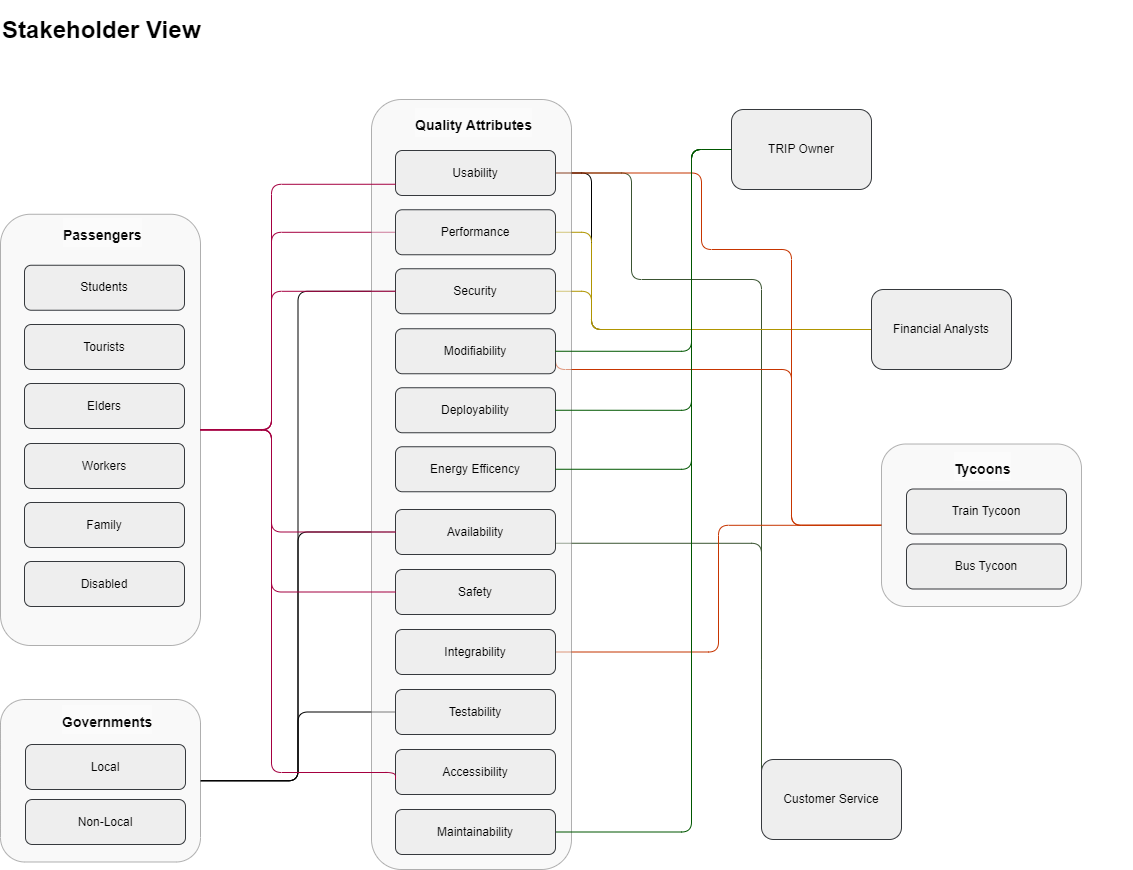
\includegraphics[width=\textwidth]{drawings/views_final_version/stakeholder_view.png}
    \caption{Stakeholder model of the TRIP system.}
    \label{fig:stakeholder_view_model}
\end{figure}

\subsubsection{Description}
The Stakeholder View of the TRiP System identifies the main participants and the corresponding quality attributes that are critical to their interaction with the system. Each stakeholder group—comprising Passengers, Tycoons, the TRiP Owner, Financial Analysts, Customer Service, and Governments—is associated with specific quality attribute depicted in the view.
\subsubsection{Glossary of Elements}
\begin{table}[H]
    \centering
    \begin{tabular}{@{}clp{9cm}@{}}
    \toprule
    \textbf{Id} & \textbf{Name} & \textbf{Description} \\
    \midrule
    1 & Passengers & Individuals or groups utilizing the TrIP system for travel, including diverse demographics such as students, tourists, workers, families, the elderly, and disabled persons. \\
    2 & Governments & Local and non-local government entities that oversee transportation regulations, public welfare, and infrastructure as it relates to the TrIP system. \\
    3 & Quality Attributes & Characteristics of the TrIP system valued by stakeholders, including usability, performance, security, modifiability, cost efficiency, availability, safety, integrability, and maintainability. \\
    4 & TRIP Owner & The entity or group of entities responsible for the oversight, strategic decision-making, and financial aspects of the TrIP system. \\
    5 & Financial Analysts & Professionals who assess the financial performance, cost-effectiveness, and economic impact of the TrIP system. \\
    6 & Tycoons & Operators or owners of train and bus services who use the TrIP system for fare collection, service management, and customer engagement. This includes both train tycoons and bus tycoons. \\
    7 & Customer Service & The support infrastructure that addresses user inquiries, resolves travel and payment issues, and enhances the overall customer experience within the TrIP system. \\
    \bottomrule
    \end{tabular}
    \caption{Glossary of stakeholder-related elements detailing the parties involved with the TrIP system and their interests.}
    \label{tab:glossary_stakeholder_view}
\end{table}


\subsection{View: Context diagram}
\subsubsection{Model}
\begin{figure}[H]
    \centering
    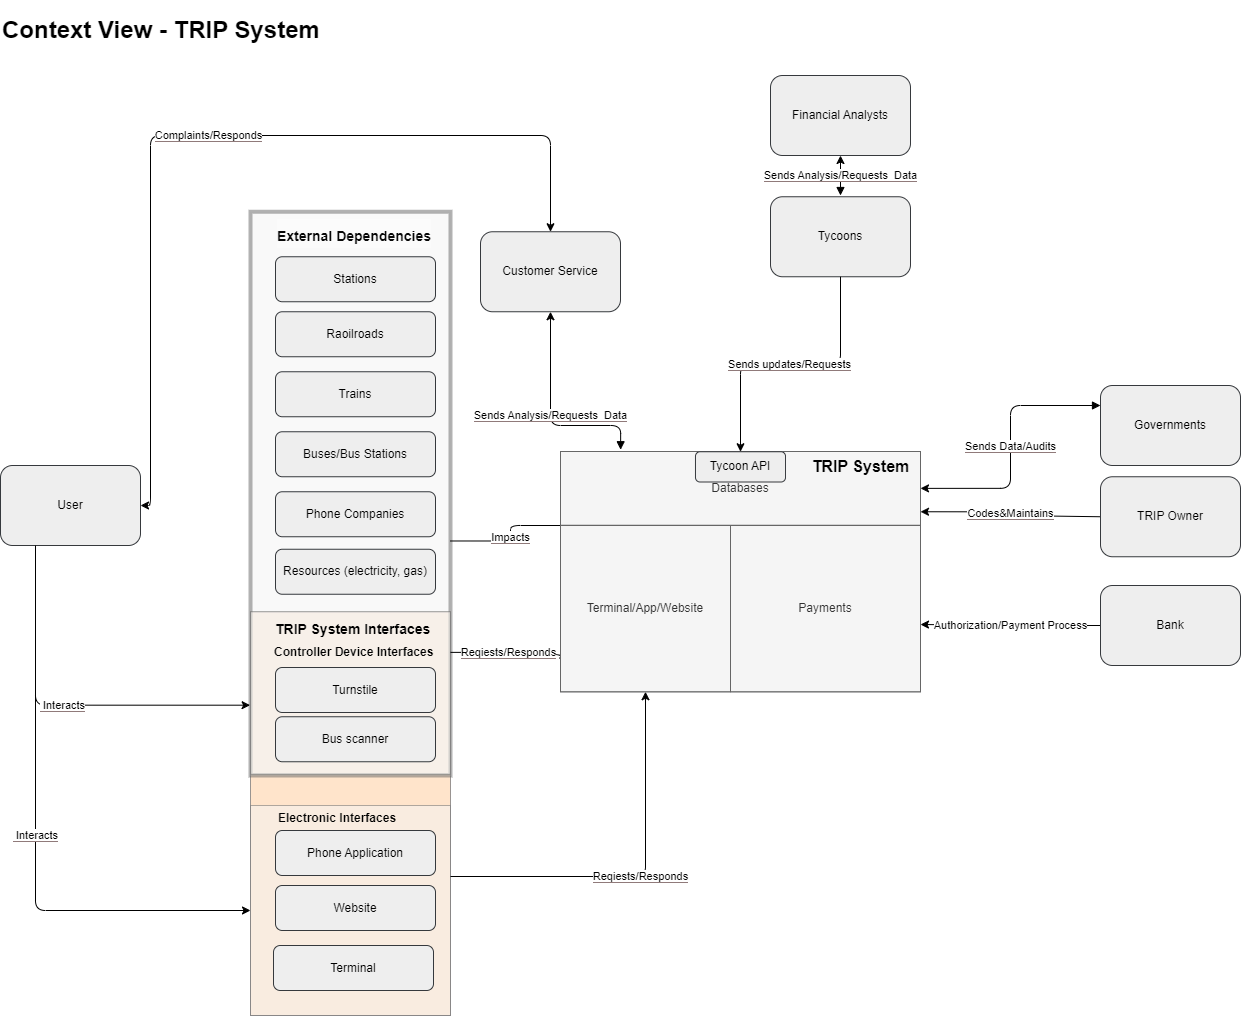
\includegraphics[width=\textwidth]{drawings/views_final_version/context_view.png}
    \caption{Context model of the TrIP system.}
    \label{fig:context_view_model}
\end{figure}

\subsubsection{Description}
The Context View of the TRiP SYSTEM delineates the ecosystem within which the system operates, including its interactions with users, external entities, and other system components. At the user level, engagement with the TRiP system is facilitated through various interfaces such as terminals, apps, websites, and controller devices like turnstiles and bus scanners, enabling passengers to access services seamlessly.

The system is subject to a range of external dependencies, including infrastructure elements like stations, railroads, and trains, as well as service providers such as phone companies and utilities that supply essential resources. These components are integral to the system's operations, impacting its functionality and performance.

At the core, the TRiP system is interconnected with Tycoons via the Tycoon API, through which data flows bidirectionally, allowing for the exchange of updates, requests, and analytical data. The databases within the system are pivotal in managing schedules, user accounts, tickets, and payments, all of which are crucial for the day-to-day operations.

The system's architecture is designed to ensure robustness and responsiveness to both the passengers' and Tycoons' needs. It facilitates various processes, from payment transactions, which are securely handled and routed through financial institutions, to the maintenance of service quality, overseen by the TRiP owner and regulated by governmental audits and codes. This comprehensive network of interactions defines the TRiP system's context, emphasizing its multifaceted nature and the critical role it plays in serving its stakeholders.

\subsubsection{Glossary of the Elements}
\begin{table}[H]
\centering
\begin{tabular}{@{}clp{9cm}@{}}
\toprule
\textbf{Id} & \textbf{Name} & \textbf{Description} \\
\midrule
1 & Passenger & Individuals who use the TrIP SYSTEM and its associated services, interacting through various interfaces. \\
2 & Customer Service & The department that handles passenger complaints and feedback, providing support and sending analysis or data requests to the system. \\
3 & Financial Analysts & Experts or entities that review financial data, requiring analytical information from the system for decision-making. \\
4 & Tycoons & The operational decision-makers of the system, possibly managers or algorithms that control system parameters and require data. \\
5 & Tycoon API & The programming interface through which Tycoons receive updates and send requests to the system. \\
6 & TrIP System & The core system that integrates various interfaces and processes, forming the central operation platform. \\
7 & Governments & Regulatory bodies that may require data or perform audits on the system for governance and compliance. \\
8 & TrIP Owner & The entity or person owning and maintaining the TrIP SYSTEM, responsible for its overall functionality. \\
9 & Bank & Financial institution that handles the authorization and processing of payments for the system. \\
10 & Stations & Locations where the TrIP SYSTEM provides service to passengers, such as train or bus stations. \\
11 & Railroads & Infrastructure providers that offer the tracks on which train services operate. \\
12 & Trains & The vehicles used by the system to transport passengers from one station to another. \\
13 & Buses/Bus Stations & The bus services and their stations that are part of the transport network. \\
14 & Phone Companies & Telecom service providers that facilitate mobile communication and data transfer for the system. \\
15 & Resources (electricity, gas) & Utility providers that supply essential power and energy required for the system’s operations. \\
16 & Controller Device Interfaces & The interfaces like turnstiles and bus scanners that manage access control and validate user credentials. \\
17 & Electronic Interfaces & Digital platforms such as mobile applications and websites that passengers interact with for services. \\
\bottomrule
\end{tabular}
\caption{Context model glossary for the TrIP System.}
\label{tab:glossary_context_view}
\end{table}

% Scenario 1: Usability Enhancement through Standardized UIs
\begin{table}[H]
    \centering
    \begin{tabularx}{\textwidth}{@{} lX @{}}
    \toprule
    \textbf{Aspect} & \textbf{Details} \\
    \midrule
    Source & Passenger interacts with the payment terminal UI. \\
    Stimulus & The passenger navigates the options to buy a ticket. \\
    Artifact & Standardized User Interface (UI) of the payment terminal. \\
    Response & The UI displays a clear, consistent, and intuitive navigation path for ticket purchase. \\
    Measure & 95\% of passengers successfully purchase tickets without assistance. \\
    \bottomrule
    \end{tabularx}
    \caption{Scenario for Usability - Standardized UIs}
    \label{table:usability_enhancement}
\end{table}


% Scenario 2: Scalability via Tycoon API
\begin{table}[H]
    \centering
    \begin{tabularx}{\textwidth}{@{} lX @{}}
    \toprule
    \textbf{Aspect} & \textbf{Details} \\
    \midrule
    Source & A new tycoon's system attempting to integrate with the TrIP system. \\
    Stimulus & The tycoon sends a request to access route and fare data. \\
    Artifact & Tycoon API that standardizes data exchange with the TrIP system. \\
    Response & The API facilitates the integration, providing access to the required data. \\
    Measure & Integration is completed within 3 business days, with zero errors in data format conversion. \\
    \bottomrule
    \end{tabularx}
    \caption{Scenario for Scalability via Tycoon API}
    \label{table:scalability_tycoon_api}
\end{table}

% Scenario: Payment Flexibility for Diverse User Groups
% Scenario: Accommodating Varied Payment Preferences
\begin{table}[H]
    \centering
    \begin{tabularx}{\textwidth}{@{} lX @{}}
    \toprule
    \textbf{Aspect} & \textbf{Details} \\
    \midrule
    Source & Passengers with varying preferences for payment, each approaching the transit system's access points. \\
    Stimulus & Passengers select their payment method of choice, ranging from physical cash for single rides to digitally managed subscriptions, and some opt for the convenience of pre-loaded fare cards. \\
    Artifact & Integrated payment and authentication platform within the TrIP system. \\
    Response & The system adeptly manages the assortment of transactions, crediting cash payments, verifying subscription validity, and debiting pre-loaded cards, all in a streamlined fashion. \\
    Measure & The system consistently processes transactions of all types with a rapid response rate, registering a less than 2-second average processing time and maintaining a transaction success rate of 99\%. \\
    \bottomrule
    \end{tabularx}
    \caption{Scenario for Usability via Accommodating Varied Payment Preferences}
    \label{table:varied_payment_preferences}
\end{table}

\section{Functional Viewpoint}

We start discussing the Functional Viewpoint by analyzing stakeholder concerns that need to be addressed.
We individuated the following user stories:
\begin{itemize}
    \item User stories TODO
\end{itemize}

As a consequence, we decided to prioritize Quality Attributes for this view as indicated in Table~\ref{tab:functional_view}.
\begin{table}[h!]
    \centering
    \resizebox{\textwidth}{!}{%
    \begin{tabular}{|l|c|c|c|c|c|c|c|c|c|}
      \hline
      & Usability & Performance & Security & Modifiability & Cost Efficiency & Availability & Safety & Integrability & Maintainability \\
      \hline
      Functional View & 
      \cellcolor{gray!60}X & % Usability (2nd priority)
      \cellcolor{gray!40}X & % Performance (3rd priority)
      & & 
      \cellcolor{gray!55}X & % Cost (3rd priority)
      & % Availability (4th priority)
      & 
      \cellcolor{gray!20}X& 
      \cellcolor{gray!90}X \\ % Maintainability (1st priority)
      \hline
    \end{tabular}
    }
    \caption{Functional View Prioritized Quality Attributes}
    \label{tab:functional_view}
\end{table}


\subsection{View: Main Functional Elements}

\subsubsection{Model}

\begin{figure}[H]
    \centering
    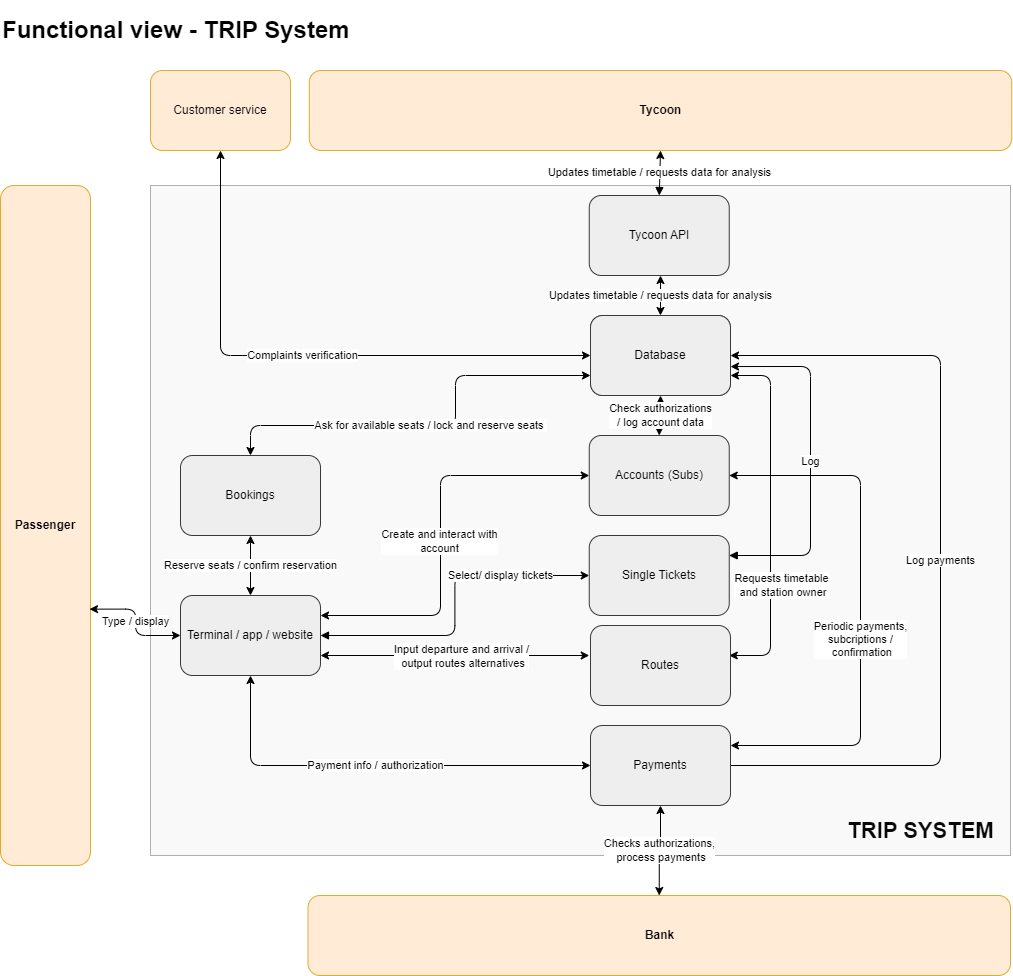
\includegraphics[width=\textwidth]{drawings/views_final_version/functional_view.png}
    \caption{TrIP System.}
    \label{fig:trip_system}
\end{figure}

\subsubsection{Description}
The functional view diagram of the TrIP system illustrates the major functions of the system and how they interact with each other. The diagram features boxes representing different functions, connected by arrows that represent interactions.
The system starts with the user, who can interact with the system through various interfaces, such as terminals, apps, or websites. The user can input their departure and arrival stations, and the system will then display a list of available routes. The user can then select a route and proceed to payment.
The payment system can handle various payment methods, including single tickets, subscriptions, and fillable cards. If the user has a subscription, the system will automatically check if the subscription is valid for the selected route. This is done by the Account and Subscription Management module, which communicates with the tycoon systems to verify the subscription. If the subscription is not valid, the user will be prompted to purchase a single ticket or top up their fillable card.
Once the payment is processed, the system will generate a ticket or update the user's travel card. The user can then scan their ticket or card at the turnstile to gain access to the train platform. The turnstile communicates with the Account and Subscription Management module to verify the ticket or card and update the passenger's state.
The system also includes a number of other functions, such as a booking system, a route optimization system, and a customer service system. The booking system allows users to reserve seats on trains. The route optimization system helps users find the most efficient routes between their departure and arrival stations. The customer service system provides support to passengers with inquiries and complaints.
The system is designed to be scalable and flexible, so that it can be easily adapted to accommodate new tycoons and changing business models. The system is also designed to be secure, so that passenger data is protected from unauthorized access.

\subsubsection{Glossary of Elements}
\begin{table}[H]
    \centering
    \begin{tabular}{@{}clp{9cm}@{}}
    \toprule
    \textbf{Id} & \textbf{Name} & \textbf{Description} \\
    \midrule
    1 & Passenger & End-users of the TrIP SYSTEM who interact with various system components to manage their travel experience. \\
    2 & Customer Service & The interface for passengers to make inquiries or complaints and receive assistance with bookings or account issues. \\
    3 & Tycoon & The administrative or business logic module that updates timetables and analyzes system data for improvements or reporting. \\
    4 & Database & An abstraction for the set of databases that stores all system data including passenger accounts, bookings, and payment information. Detailed information about how different databases are handled is detailed in the Information View.\\
    5 & Bookings & The system component where passengers can inquire about seat availability and make reservations. \\
    6 & Accounts (Subs) & The system managing passenger accounts and subscriptions, responsible for authorization checks and account data logging. 
    It is is also responsible for single tickets and fillable cards, as they can be seen as temporary and anonymous accounts. \\
    7 & Routes & The component that manages route information and provides passengers with timetables, station ownership details, and route alternatives. \\
    8 & Payments & The module handling all financial transactions, including passenger payments and periodic billing. \\
    9 & Bank & The financial institution interface for authorizing and processing payments linked to the system. \\
    10 & Terminal/App/Website & User interfaces through which they can access services such as booking, route information, and payment. \\
    \bottomrule
    \end{tabular}
    \caption{Glossary of elements detailing the components of the TrIP SYSTEM and their roles in facilitating user interaction and service provision.}
    \label{tab:glossary_trip_system}
\end{table}

\subsubsection{Analysis on Perspectives}
In addressing the Quality Attribute (QA) priorities highlighted by users, our Main Functional Elements view incorporates several key decisions designed to enhance usability, maintainability, scalability, and performance efficiency. \\

\noindent \textbf{Scenarios}
\scenarioOneFunctional
\scenarioTwoFunctional

\noindent To meet the \textit{usability} needs of passengers, we have opted for standardized User Interfaces (UIs). These UIs, being open-source and widely utilized, benefit from a large user base that contributes to their \textit{maintenance} and robustness. This choice ensures a user-friendly and reliable interface for passengers over the long term. Furthermore, it aligns with the TrIP owner's preferences by offering ease of maintenance and \textit{low operational costs}.

In response to Event 1, which underscored the need for easier \textit{integration} of new tycoons, we have implemented the Tycoon API. This API standardizes data requests from each tycoon, irrespective of their mode of transportation, thus facilitating the smooth integration of new tycoons into the system. The Tycoon API, in conjunction with the accounts and bookings module, ensures that passengers can effortlessly utilize their subscriptions across different networks and book their preferred routes. Hence, implementation of Tycoon API increases the \textit{usability} and \textit{integrability} for the Tycoons.

Event 3, which focused on traffic jams, raised the importance of optimizing system \textit{performance} during peak periods. By deciding on a centralized route management module, we have streamlined data flow between the TrIP system and the tycoons. This module not only simplifies data management but also enhances the system's ability to handle high request volumes through optimization and caching strategies.

\subsection{View: Ticket scanning}
\subsubsection{Model}
\begin{figure}[H]
    \centering
    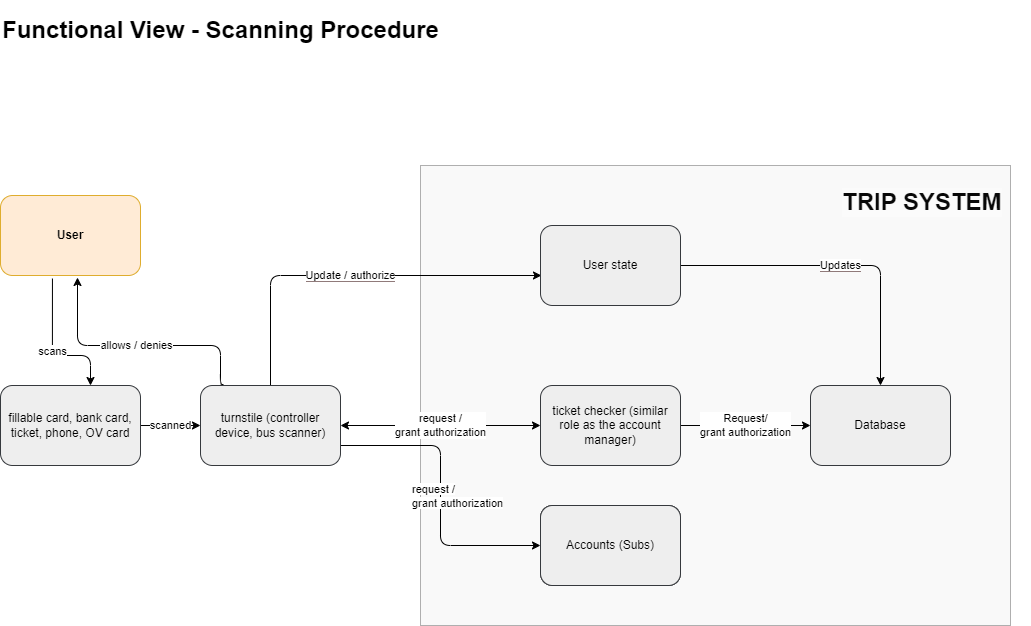
\includegraphics[width=\textwidth]{drawings/views_final_version/functional_view scanning.png}
    \caption{Interaction with a ticket scanner.}
    \label{fig:ticket_scanner}
\end{figure}

\subsubsection{Description}
The scanning procedure within the TRIP SYSTEM encapsulates the interactions between the passenger and the system's access control mechanisms. It begins with the user presenting a valid form of transit access—such as a card or mobile device—to a scanning device like a turnstile or bus scanner. This device then consults the User state, a repository of the passenger's authorization status, to allow or deny entry. In parallel, the Ticket Checker function verifies the user's credentials against the Accounts subsystem, which manages detailed account information and subscriptions. Any changes to the user's status are updated in real time in the central Database, ensuring accurate tracking of access and travel history. This process ensures a secure, streamlined experience for passengers while providing the system with the necessary oversight to prevent unauthorized access

\subsubsection{Glossary of Elements}
\begin{table}[H]
    \centering
    \begin{tabular}{@{}clp{9cm}@{}} % Adjust the width of the description column as needed to fit the page
    \toprule
    \textbf{Id} & \textbf{Name} & \textbf{Description} \\
    \midrule
    1 & Passenger & The individual who uses the trip system and interacts with various components such as turnstiles and ticket checkers. \\
    2 & Fillable Card, Bank Card, Ticket, Phone, OV Card & Various forms of identification or payment methods that the passenger can use within the system. These are scanned by the turnstile to allow or deny access. \\
    3 & Turnstile (Controller Device, Bus Scanner) & A physical barrier or scanner that reads the passenger's ticket or card and determines whether to grant or deny access based on the passenger state or account information. \\
    4 & Passenger State & A system component that maintains the current state of the passenger within the system, including authorization and access rights, which is updated upon passenger interaction with the turnstile. \\
    5 & Ticket Checker (Account Manager) & An agent or system role similar to the account manager that requests or grants authorization for passenger access, potentially by checking the passenger state against the database. \\
    6 & Accounts (Subs) & The subsystem managing passenger accounts and subscriptions, which may interact with the turnstile and ticket checker to verify and update passenger access rights. \\
    7 & Database & An abstraction for the set of databases that stores all system data including passenger accounts, bookings, and payment information. Detailed information about how different databases are handled is detailed in the Information View.\\
    \bottomrule
    \end{tabular}
    \caption{Glossary of elements for the Functional View - Turnstiles, detailing the components and their roles in passenger access and authorization within the TrIP SYSTEM.}
    \label{tab:glossary_turnstiles}
\end{table}

\subsubsection{Analysis on Perspectives}
In addressing the Quality Attribute (QA) priorities highlighted by users, our ticket scanning view incorporates several key decisions designed to enhance usability, maintainability, scalability, and performance efficiency.

The introduction of multiple payment methods, including fillable cards, credit cards, and single tickets, significantly simplifies passenger interaction with the TrIP system. The integration of accounts and subscriptions further facilitates seamless travel across multiple tycoon networks, enabling passengers to efficiently manage and use their subscriptions.

\paragraph{Scenarios}
\scenarioThreeFunctional

In summary, the functional viewpoint of our system meticulously addresses the initial QA priorities, along with the challenges presented by new tycoon integration (Event 1) and traffic jams (Event 3). These decisions collectively ensure a user-friendly, scalable, and high-performing TrIP system for passengers, tycoons, and the TrIP owner alike.
% Scenario: Protecting Passenger Personal and Travel Information
\newcommand{\scenarioOneInformation}{
\begin{table}[H]
    \centering
    \begin{tabularx}{\textwidth}{@{} lX @{}}
    \toprule
    \textbf{Aspect} & \textbf{Details} \\
    \midrule
    Source & Passenger utilizing the TrIP system to manage their travel plans. \\
    Stimulus & The passenger enters personal and travel data into the system. \\
    Artifact & Encrypted Account Lookup Database within the TrIP system. \\
    Response & The system securely stores the passenger's data using state-of-the-art encryption both at rest and in transit, ensuring that personal and travel information is not accessible by unauthorized entities. Access to this data is restricted to specific operations within the TrIP system that require passenger verification. \\
    Measure & Passenger data breaches are non-existent, and passengers report a high level of trust in the system's data protection capabilities. Security logs show no unauthorized access, affirming the integrity of the encryption measures. \\
    \bottomrule
    \end{tabularx}
    \caption{Scenario for Security - Passenger Data Protection}
    \label{table:passenger_data_security}
\end{table}
}

% Scenario: Secure Payment Processing for Passenger Transactions
\newcommand{\scenarioTwoInformation}{
\begin{table}[H]
    \centering
    \begin{tabularx}{\textwidth}{@{} lX @{}}
    \toprule
    \textbf{Aspect} & \textbf{Details} \\
    \midrule
    Source & Passenger making a payment through the TrIP system. \\
    Stimulus & The passenger chooses a payment method and initiates a transaction. \\
    Artifact & Bank interfaced with TrIP system for processing payments. \\
    Response & The bank processes the payment with rigorous security protocols, ensuring that the payment information is handled in a secure, encrypted channel. The system guarantees that payment data is never stored within the TrIP system and is managed exclusively by the bank, providing an additional layer of security. \\
    Measure & Payment transactions are completed with zero incidents of data compromise, and the response time for transaction completion remains within 3 seconds. Post-transaction audits confirm the absence of payment data retention within the TrIP system. \\
    \bottomrule
    \end{tabularx}
    \caption{Scenario for Security - Secure Payment Transactions}
    \label{table:payment_transaction_security}
\end{table}
}

% Scenario: Controlled Access to Passenger Account Data
\newcommand{\scenarioThreeInformation}{
\begin{table}[H]
    \centering
    \begin{tabularx}{\textwidth}{@{} lX @{}}
    \toprule
    \textbf{Aspect} & \textbf{Details} \\
    \midrule
    Source & Passenger subscribing to a specific tycoon's services within the TrIP system. \\
    Stimulus & The subscribed tycoon requests access to the passenger's account data for service personalization. \\
    Artifact & Tycoon API enabling access control to passenger data within the TrIP system. \\
    Response & The TrIP system authenticates the tycoon's request through the Tycoon API, which validates that only the tycoon with whom the passenger is subscribed can retrieve the required data. This ensures that each tycoon can access only their passengers’ data, thus maintaining strict data access control and privacy. \\
    Measure & Regular audits indicate 100\% compliance with data access policies, with no reported incidents of data leakage or unauthorized access. Passenger feedback confirms trust in the data privacy practices of the TrIP system. \\
    \bottomrule
    \end{tabularx}
    \caption{Scenario for Security - Controlled Tycoon Access to Passenger Data}
    \label{table:tycoon_access_control}
\end{table}
}

\section{Information Viewpoint}
We start discussing the Information Viewpoint by analyzing stakeholder concerns that need to be addressed.
We individuated the following user stories:
\begin{itemize}
    \item User stories TODO
\end{itemize}

As a consequence, we decided to prioritize Quality Attributes for this view as indicated in Table~\ref{tab:information_view}.

\begin{table}[h!]
    \centering
    \resizebox{\textwidth}{!}{%
    \begin{tabular}{|l|c|c|c|c|c|c|c|c|c|}
      \hline
      & Usability & Performance & Security & Modifiability & Cost Efficiency & Availability & Safety & Integrability & Maintainability \\
      \hline
      Information View & 
       & % Usability
       & % Performance
      \cellcolor{gray!90}X & % Security (1st priority)
       & % Modifiability
       & % Cost Efficiency
       & % Availability
       & % Safety
       & % Integrability
       \\ % Maintainability
      \hline
    \end{tabular}
    }
    \caption{Information View Prioritized Quality Attributes}
    \label{tab:information_view}
\end{table}

\subsection{View: Main Information View}
\subsubsection{Model}
\begin{figure}[H]
    \centering
    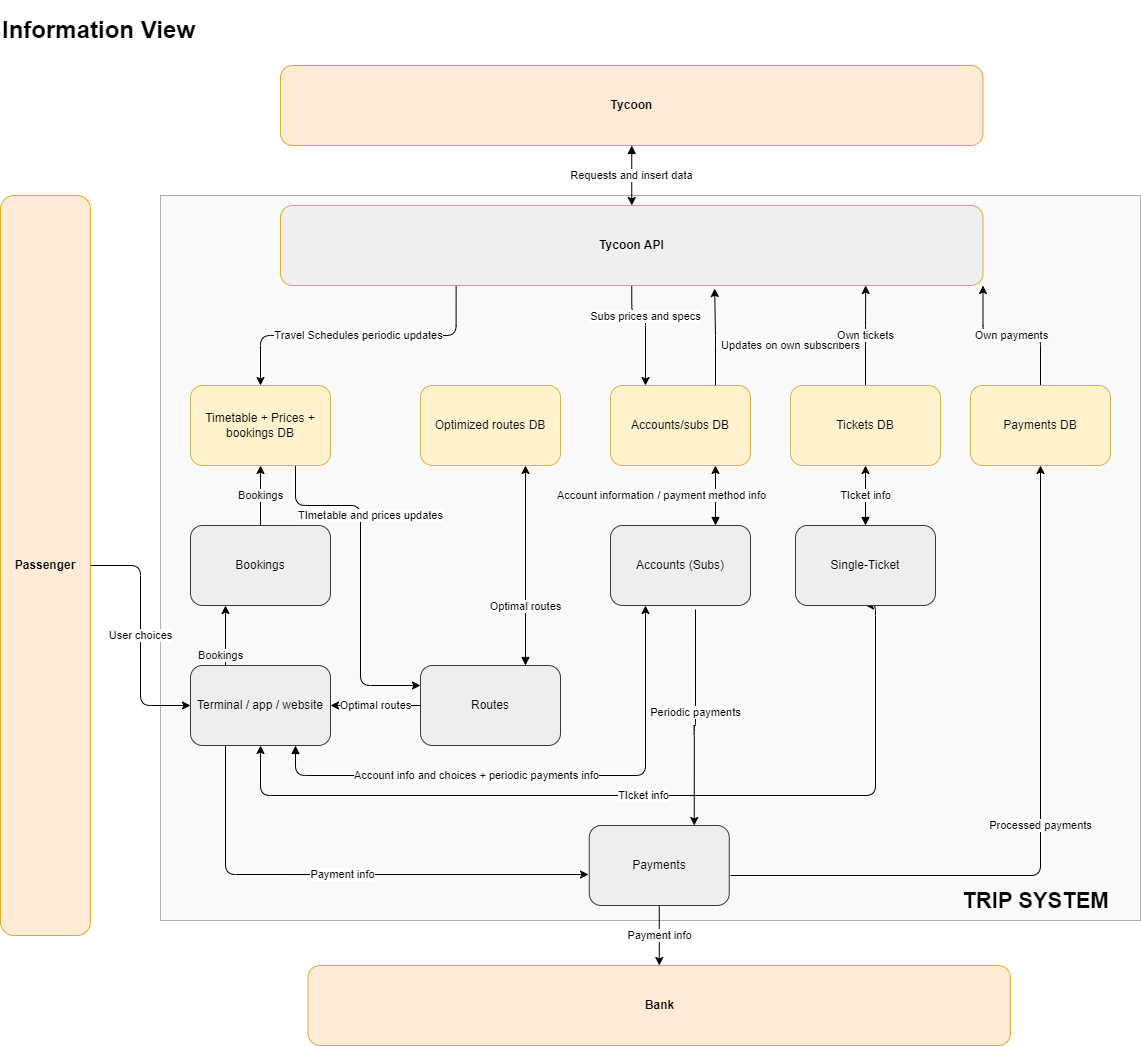
\includegraphics[width=\textwidth]{drawings/views_final_version/information_view.png}
    \caption{Information view.}
    \label{fig:information_view}
\end{figure}

\subsubsection{Description}
The Information View of the TrIP SYSTEM is about how data moves and is stored. The system uses several databases. The Timetable + Prices + Bookings DB keeps track of schedules, prices, and reservations. The Optimized Routes DB has data on the best travel paths. The Accounts/Subs DB holds information on user accounts and subscriptions. The Tickets DB records ticket purchases, and the Payments DB keeps a record of all payments.

Tycoons use the Tycoon API to put in and get data. Passengers use terminals, apps, or websites to book travel and select routes. This choice and payment info go into the databases, updating the system.

The Routes component uses the Optimized Routes DB to give passengers the best travel options. The Accounts (Subs) part handles subscription details and payments, working with the Accounts/Subs DB. For single tickets, there's a separate interface that works with the Tickets DB. Payments process transactions and send completed payment information to the bank.

\subsubsection{Glossary of Elements}

\begin{table}[H]
    \centering
    \caption{Glossary of elements for the Information View of the TrIP SYSTEM.}
    \label{tab:information_view_glossary}
    \begin{tabularx}{\textwidth}{@{}lX@{}} % Use 'X' for auto-adjusting width
    \toprule
    \textbf{Element} & \textbf{Description} \\
    \midrule
    Tycoon & Tycoons responsible for making requests for analysis, and inserting travel data. \\
    Tycoon API & Tycoon's way of interacting to the TrIP system. \\
    Timetable + Prices + bookings DB & Stores data regarding travel schedules, pricing, and booking information. \\
    Optimized routes DB & Contains information on the most efficient travel routes that have been calculated and stored. \\
    Accounts/Subs DB & Maintains records of user accounts and their subscriptions for travel services. \\
    Tickets DB & A database that logs ticket purchases and holds ticket-related information. \\
    Payments DB & Records and processes transactions related to payments within the system. \\
    Passenger & The end-user or customer who utilizes the system for travel services. \\
    Bookings & The system component or interface that passengers interact with to manage and view their bookings. \\
    Terminal / App / Website & The various platforms through which passengers can access the system for services. \\
    Routes & Involves the determination and selection of travel routes within the system. \\
    Accounts (Subs) & Manages the subscription details associated with user accounts. \\
    Single-Ticket & A system or interface that deals with the purchase of individual travel tickets. \\
    Periodic payments & Manages recurring payments, typically for subscription services. \\
    Payments & Processes transactions related to immediate payments within the system. \\
    Processed payments & A log or record of payment transactions that have been completed. \\
    Bank & The financial institution where final payment transactions are processed and funds are transferred. \\
    \bottomrule
    \end{tabularx}
\end{table}

\subsubsection{Analysis on Perspectives}
\paragraph{Scenarios}
\scenarioOneInformation
\scenarioTwoInformation
\scenarioThreeInformation

The Information View of the TrIP system provides a comprehensive architecture designed to handle and safeguard data movement and storage, ensuring the system's integrity and security.

The design segregates data across specialized databases, including those for Timetables + Prices + Bookings, Optimized Routes, Accounts/Subs, Tickets, and Payments. This segregation follows best practices in database security, preventing any single point of compromise and ensuring each database only holds data relevant to its function. Access to these databases is strictly regulated, with the system enforcing robust authentication and authorization mechanisms to verify and control interactions.

Encryption plays an important role in the system, particularly within the Accounts/Subs Database. It protects sensitive passenger information by using encrypted account lookup database. Data at rest within this database, as well as data in transit to and from it, is encrypted, thereby securing personal and travel information from unauthorized access.

Payments are a critical interaction point for the system and its users. The TrIP system approaches this by interfacing directly with banks for payment processing. This interface means that the sensitive financial information is managed within the secure domain of banking institutions, which are inherently designed to handle such data securely. This direct interfacing also implies that the TrIP system does not store payment details, which greatly reduces its liability and exposure to financial data breaches.

The Tycoon API serves as a broker for data access by tycoons. It provides a controlled access point, permitting only authorized tycoons to retrieve passenger data. This access control mechanism is crucial for maintaining passenger privacy and data security. It allows tycoons to access only the data necessary for their service offerings and nothing beyond that.

Using the scenarios provided, we can see how the system's design and technology choices map directly to its operations. Passengers entering their information into terminals or apps can be assured that their data will be encrypted and stored securely, as detailed in the first scenario. Payment processes, as per the second scenario, happen within the secure confines of the banking system. Lastly, the way the Tycoon API manages data requests ensures that passenger data is only accessed by authorized tycoons, enhancing privacy and data protection as outlined in the third scenario.
\subsection{View: Scanning information flows}
\subsubsection{Model}
\begin{figure}[H]
    \centering
    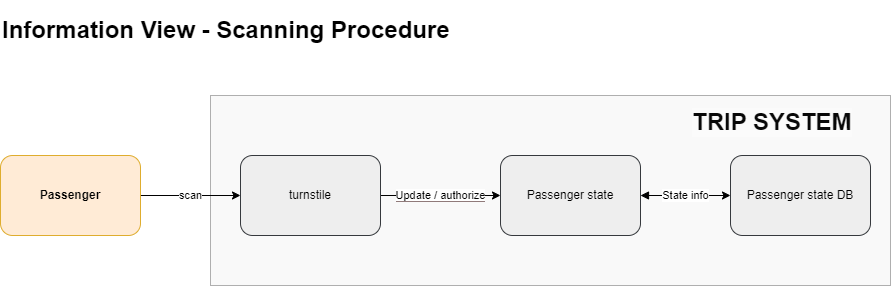
\includegraphics[width=\textwidth]{drawings/views_final_version/information_view scanning.png}
    \caption{Information view related to the scanning procedure.}
    \label{fig:information_view_scanning}
\end{figure}

\subsubsection{Description}
The TrIP SYSTEM's scanning procedure is a sequence that starts with the Passenger, who scans at the Turnstile to gain entry. This triggers the Update/Authorize process, updating the Passenger State with the user's access rights. The Passenger State reflects the user's current permissions within the TRIP SYSTEM. Each user’s information is recorded in the Passenger State DB, a database that tracks and manages user statuses.

\begin{table}[H]
    \centering
    \caption{Legend for the Scanning Procedure in the Information View of the TrIP SYSTEM.}
    \label{tab:scanning_procedure_legend}
    \begin{tabular}{@{}llp{10cm}@{}}
    \toprule
    \textbf{Id} & \textbf{Name} & \textbf{Description} \\
    \midrule
    1 & Passenger & The starting point representing the individual using the TrIP SYSTEM. \\
    2 & Turnstile & The physical or virtual entry point where the passenger scans to gain access. \\
    3 & Update / Authorize & The process that updates the system and authorizes the passenger to proceed. \\
    4 & Passenger State & The current status of the passenger within the system, which is updated after scanning. \\
    5 & Passenger State DB & The database that records the state information of the passenger. \\
    \bottomrule
\end{tabular}
\end{table}

\subsubsection{Analysis on Perspectives}



% Scenario: Ensuring Service Availability During Network Outages
\newcommand{\scenarioOneConcurrency}{
\begin{table}[H]
    \centering
    \begin{tabularx}{\textwidth}{@{} lX @{}}
    \toprule
    \textbf{Aspect} & \textbf{Details} \\
    \midrule
    Source & Network outage impacting the TrIP system's connectivity. \\
    Stimulus & A passenger attempts to validate their ticket at a turnstile during the outage. \\
    Artifact & Hybrid approach of delayed processing and local caching implemented in the TrIP system. \\
    Response & The turnstile, equipped with local caching, validates the passenger's ticket against stored data, allowing entry. Transaction details are queued for delayed processing once network connectivity resumes, ensuring no service disruption. \\
    Measure & Passenger service continuity is maintained with 99.9\% uptime, and ticket validations during outages show no significant delay, ensuring high system availability. \\
    \bottomrule
    \end{tabularx}
    \caption{Scenario for Availability - Network Outage Handling}
    \label{table:availability_network_outage}
\end{table}
}
% Scenario: Maintaining Safety through Authorized Access

\newcommand{\scenarioTwoConcurrency}{
\begin{table}[H]
    \centering
    \begin{tabularx}{\textwidth}{@{} lX @{}}
    \toprule
    \textbf{Aspect} & \textbf{Details} \\
    \midrule
    Source & TrIP system's safety protocols for access control. \\
    Stimulus & An individual attempts to access the transit system without a valid ticket or permission. \\
    Artifact & Turnstile with integrated validation system that checks for valid tickets. \\
    Response & The turnstile denies entry to the individual without a valid ticket, preventing unauthorized access and maintaining the safety and security of the transit environment. \\
    Measure & Zero reported incidents of unauthorized access, ensuring the safety of the transit system and its users. \\
    \bottomrule
    \end{tabularx}
    \caption{Scenario for Safety - Authorized Access Enforcement}
    \label{table:safety_authorized_access}
\end{table}
}

% Scenario: Optimizing Performance with Pre-stored Routes
\newcommand{\scenarioThreeConcurrency}{
\begin{table}[H]
    \centering
    \begin{tabularx}{\textwidth}{@{} lX @{}}
    \toprule
    \textbf{Aspect} & \textbf{Details} \\
    \midrule
    Source & Passenger requests the best route options via the TrIP system during peak hours. \\
    Stimulus & High demand for route information causes potential strain on the system. \\
    Artifact & Optimized Routes Database that stores frequently requested route data. \\
    Response & The TrIP system quickly retrieves optimized route options from the pre-stored data, providing the passenger with fast and efficient service without needing to compute the routes in real-time. \\
    Measure & The response time for route information requests during peak periods remains under 2 seconds, enhancing the overall performance of the system. \\
    \bottomrule
    \end{tabularx}
    \caption{Scenario for Performance - Efficient Route Retrieval}
    \label{table:performance_route_optimization}
\end{table}
}

\section{Concurrency Viewpoint}
We start discussing the information viewpoint by analyzing stakeholder concerns that need to be addressed.
We individuated the following user stories:
\begin{itemize}
    \item User stories TODO
\end{itemize}

As a consequence, we decided to prioritize Quality Attributes for this view as indicated in Table~\ref{tab:concurrency_view}.
\begin{table}[h!]
    \centering
    \resizebox{\textwidth}{!}{%
    \begin{tabular}{|l|c|c|c|c|c|c|c|c|c|}
      \hline
      & Usability & Performance & Security & Modifiability & Cost Efficiency & Availability & Safety & Integrability & Maintainability \\
      \hline
      Concurrency View & 
       & % Usability
      \cellcolor{gray!30}X & % Performance (2nd priority)
       & % Security
       & % Modifiability
       & % Cost Efficiency
      \cellcolor{gray!90}X & % Availability (1st priority)
      \cellcolor{gray!60}X & % Safety
       & % Integrability
       \\ % Maintainability
      \hline
    \end{tabular}
    }
    \caption{Concurrency View Prioritized Quality Attributes}
    \label{tab:concurrency_view}
\end{table}

\subsection{View: Ticket purchase}
\subsubsection{Model}

\begin{figure}[H]
    \centering
    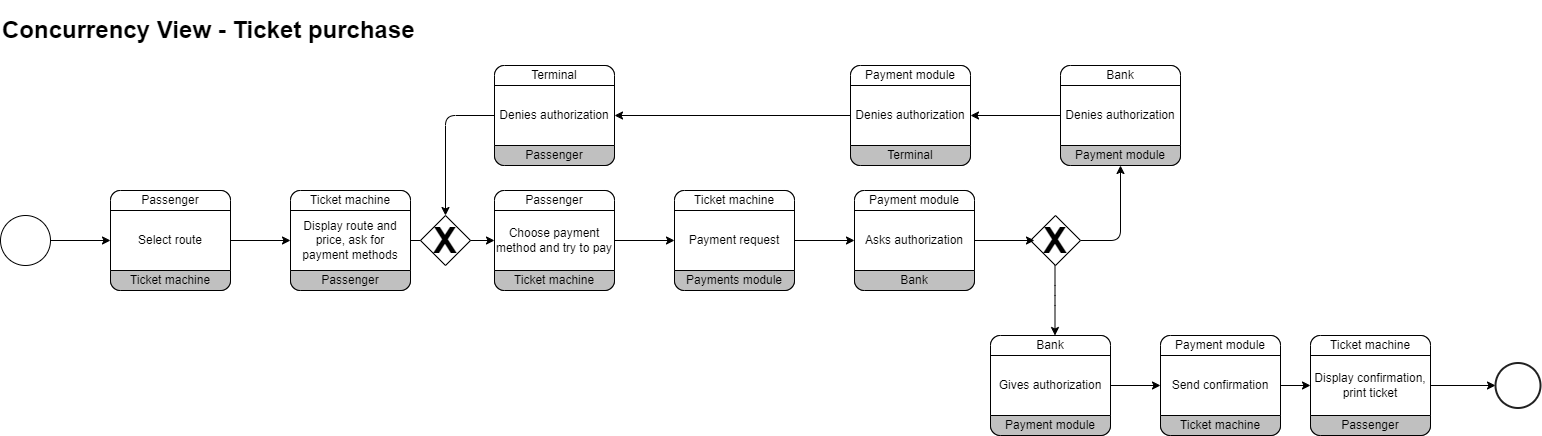
\includegraphics[width=\textwidth]{drawings/views_final_version/concurrency_view_1.png}
    \caption{Concurrency view related to ticket purchase.}
    \label{fig:concurrency_view_1}
\end{figure}

\subsubsection{Description}
In the TRIP SYSTEM, the Passenger starts the process at the Ticket Machine, choosing a route and payment method. The Terminal takes over to process the payment, and the Payment Module communicates with the Bank for payment approval. If the Bank approves, the Payment Module signals the Ticket Machine to confirm the transaction and print the ticket. If the Bank denies the payment, the process is stopped, and the Passenger is notified.

\begin{table}[H]
    \centering
    \caption{Glossary for the Payment and Ticketing Process.}
    \label{tab:payment_ticketing_glossary}
    \begin{tabularx}{\textwidth}{@{}lX@{}} % Use 'X' for auto-adjusting width
    \toprule
    \textbf{Element} & \textbf{Description} \\
    \midrule
    Passenger & The customer who initiates the process by selecting a route and choosing a payment method to pay for a ticket. \\
    Ticket Machine & The interface through which the passenger selects a route, displays the route and price, and chooses a payment method. \\
    Terminal & The point of service where the passenger's payment authorization is processed. \\
    Payment Module & The system component that interacts with the bank to request payment authorization for the transaction. \\
    Bank & The financial institution that either authorizes or denies the payment transaction. \\
    \bottomrule
    \end{tabularx}
\end{table}

\subsubsection{Analysis on Perspectives}
\textbf{Scenarios}

\scenarioThreeConcurrency

\noindent \textbf{Ticket Purchasing Process:} \\
The sequence begins with the passenger selecting a route and payment method via the Ticket Machine. This process is crucial for performance, as it demands a fast and seamless operation to prevent queues and delays. Once the payment method is chosen, the Terminal communicates with the Payment Module to process the transaction. The Payment Module's role here is two-fold: to ensure the safety of the transaction by validating payment with the bank and to maintain the system's performance by providing quick feedback to the Terminal. If the bank authorizes the payment, the Payment Module prompts the Ticket Machine to dispense a ticket, showcasing the system's availability to complete transactions without delay. In case of a denial, the passenger is promptly informed, allowing them to take alternative actions, which is vital for maintaining system usability and ensuring the passenger's experience remains positive. \\
\subsection{View: Scanning procedure}
\subsubsection{Model}
\begin{figure}[H]
    \centering
    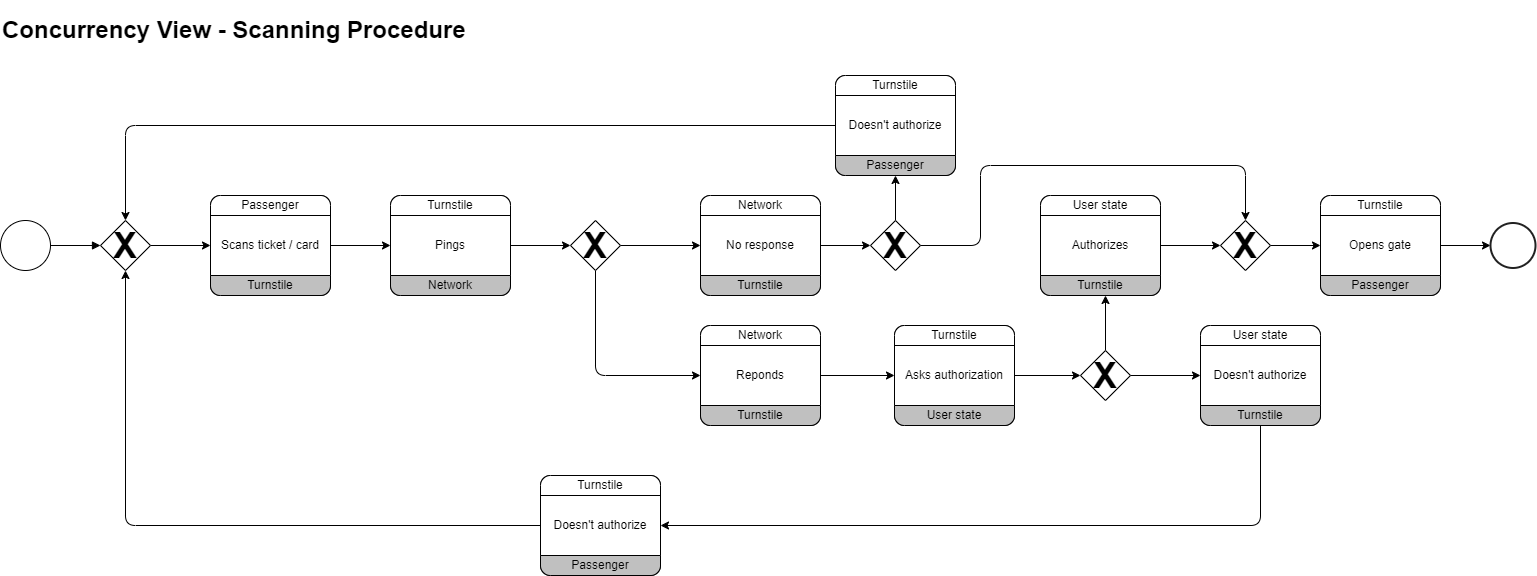
\includegraphics[width=\textwidth]{drawings/views_final_version/concurrency_view_2.png}
    \caption{Concurrency view related to the scanning procedure.}
    \label{fig:concurrency_view_2}
\end{figure}

\subsubsection{Description}
The diagram depicts a turnstile access procedure with conditional paths based on network availability and user authorization. When a Passenger scans their ticket or card at the Turnstile, two scenarios can unfold:

\begin{enumerate}
    \item If the Turnstile is unable to connect to the Network (no response), it defaults to a local decision. In this case, the turnstile can still potentially authorize the passenger to proceed based on offline data or preconfigured rules.
    \item If the Turnstile connects to the Network (network responds), it then requests authorization from the User State. The User State, after evaluating the request, either grants or denies authorization:
    \begin{itemize}
        \item If the User State authorizes the request, the Turnstile receives a signal to open the gate, allowing the Passenger to pass.
        \item If the User State denies the request, the Turnstile will not open, and the Passenger is not allowed to proceed.
    \end{itemize}
\end{enumerate}

This process ensures that the system can function and provide decisions autonomously, even in the absence of network connectivity, enhancing reliability and user experience.

\subsubsection{Glossary of Elements}

\begin{table}[H]
    \centering
    \caption{Glossary for Turnstile Interaction Process.}
    \label{tab:turnstile_interaction_glossary}
    \begin{tabularx}{\textwidth}{@{}lX@{}} % Use 'X' for auto-adjusting width
    \toprule
    \textbf{Component} & \textbf{Description} \\
    \midrule
    Passenger & An individual who is attempting to gain entry through the turnstile by scanning a ticket or card. \\
    Turnstile & A physical barrier at an entry point that controls access, typically based on ticket or card validation. \\
    Network & The communication system that the turnstile interfaces with to verify access rights. \\
    User State & A system component that maintains the current state of a user's access rights, determining whether entry is authorized. \\
    \bottomrule
    \end{tabularx}
\end{table}
\subsubsection{Analysis on Perspectives}
\textbf{Scenarios}

\scenarioOneConcurrency
\scenarioTwoConcurrency
\noindent \textbf{Turnstile Access Control:} \\
The second aspect of concurrency comes into play at the turnstiles, where passengers scan their tickets or cards to gain access to the transport services. In this operation, the system's availability and safety are the primary concerns. The Turnstile must quickly authorize entry to avoid creating bottlenecks, which it does by pinging the Network to retrieve the User State information. If the Network is unresponsive, the Turnstile uses locally cached data to make an authorization decision, ensuring continuous operation and thus maintaining high availability. When the Network responds, the User State determines access permission. This dual approach ensures that access control is robust against network issues, preserving the integrity of operations and passenger safety by preventing unauthorized access. \\
\subsection{View: Tycoon data updates}
\subsubsection{Model}

\begin{figure}[H]
    \centering
    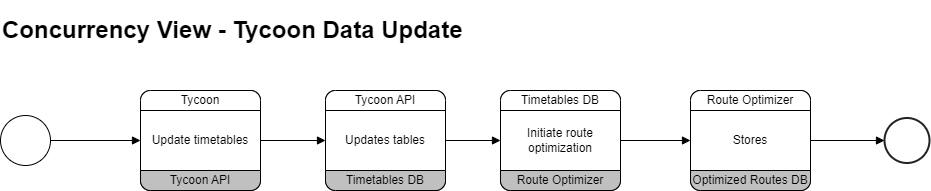
\includegraphics[width=\textwidth]{drawings/views_final_version/concurrency_view_3.png}
    \caption{Concurrency view related to tycoons data updates.}
    \label{fig:concurrency_view_3}
\end{figure}

\subsubsection{Description}
This process outlines how timetable updates and route optimization are handled in the system. It begins with the Tycoon, an administrative role, who updates timetables through the Tycoon API. These updates are then applied to the Timetables DB. Following this update, the Route Optimizer initiates the optimization process, which takes the updated timetable data to determine the most efficient routes. These optimized routes are then stored in the Optimized Routes DB, completing the cycle of updating and optimizing the route information available to the system and its users.

\begin{table}[H]
    \centering
    \caption{Glossary for Route Optimization Process.}
    \label{tab:route_optimization_glossary}
    \begin{tabularx}{\textwidth}{@{}lX@{}} % Use 'X' for auto-adjusting width
    \toprule
    \textbf{Component} & \textbf{Description} \\
    \midrule
    Tycoon & Represents the train companies or transport entities responsible for managing train schedules and routes. \\
    Tycoon API & The application programming interface that allows the tycoons to update and access timetable information. \\
    Timetables DB & The database where train schedules, routes, and associated data are stored and updated. \\
    Route Optimizer & The system component that calculates the most efficient routes, likely using algorithms to process timetable data. \\
    Optimized Routes DB & A specialized database that stores the results of the route optimization process. \\
    \bottomrule
    \end{tabularx}
\end{table}
\subsubsection{Glossary of Elements}

\subsubsection{Analysis on Perspectives}

The Concurrency Viewpoint is central to the TRiP system's architecture, focusing on ensuring that user interactions with the system occur smoothly and without delay, even when multiple operations are executed simultaneously. This viewpoint addresses the system's capacity to manage concurrent actions effectively, with a particular emphasis on maintaining performance, safety, and availability. \\

\noindent \textbf{Route Optimization Updates:} \\
Finally, the system’s capacity to update and optimize routes through the Tycoon API and Route Optimizer reflects its modifiability and performance attributes. Tycoons can update timetables, which are then processed to optimize routes, and these optimizations are stored in the Optimized Routes DB for quick retrieval. This ensures that passengers receive up-to-date and efficient routing information, which is especially important during peak traffic conditions. \\

By detailing these processes, the concurrency viewpoint showcases the TrIP system's capability to maintain a high level of service and security across its operations, aligning with the defined quality attributes of performance, safety, and availability.
\section{Deployment Viewpoint}
We start discussing the information viewpoint by analyzing stakeholder concerns that need to be addressed.
We individuated the following user stories:
\begin{itemize}
    \item User stories TODO
\end{itemize}

As a consequence, we decided to prioritize Quality Attributes for this view as indicated in Table~\ref{tab:deployment_view}.
\begin{table}[h!]
    \centering
    \resizebox{\textwidth}{!}{%
    \begin{tabular}{|l|c|c|c|c|c|c|c|c|c|}
      \hline
      & Usability & Performance & Security & Modifiability & Cost Efficiency & Availability & Safety & Integrability & Maintainability \\
      \hline
      Deployment View & 
       & % Usability
      \cellcolor{gray!90}X & % Performance (1st priority)
      \cellcolor{gray!60}X & % Security (3rd priority)
       & % Modifiability
       & % Cost Efficiency
       & % Availability (2nd priority)
       & % Safety
       & % Integrability
       \\ % Maintainability
      \hline
    \end{tabular}
    }
    \caption{Deployment View Prioritized Quality Attributes}
    \label{tab:deployment_view}
\end{table}

\subsection{View: Scanning procedure}
\subsubsection{Model}
\begin{figure}[H]
    \centering
    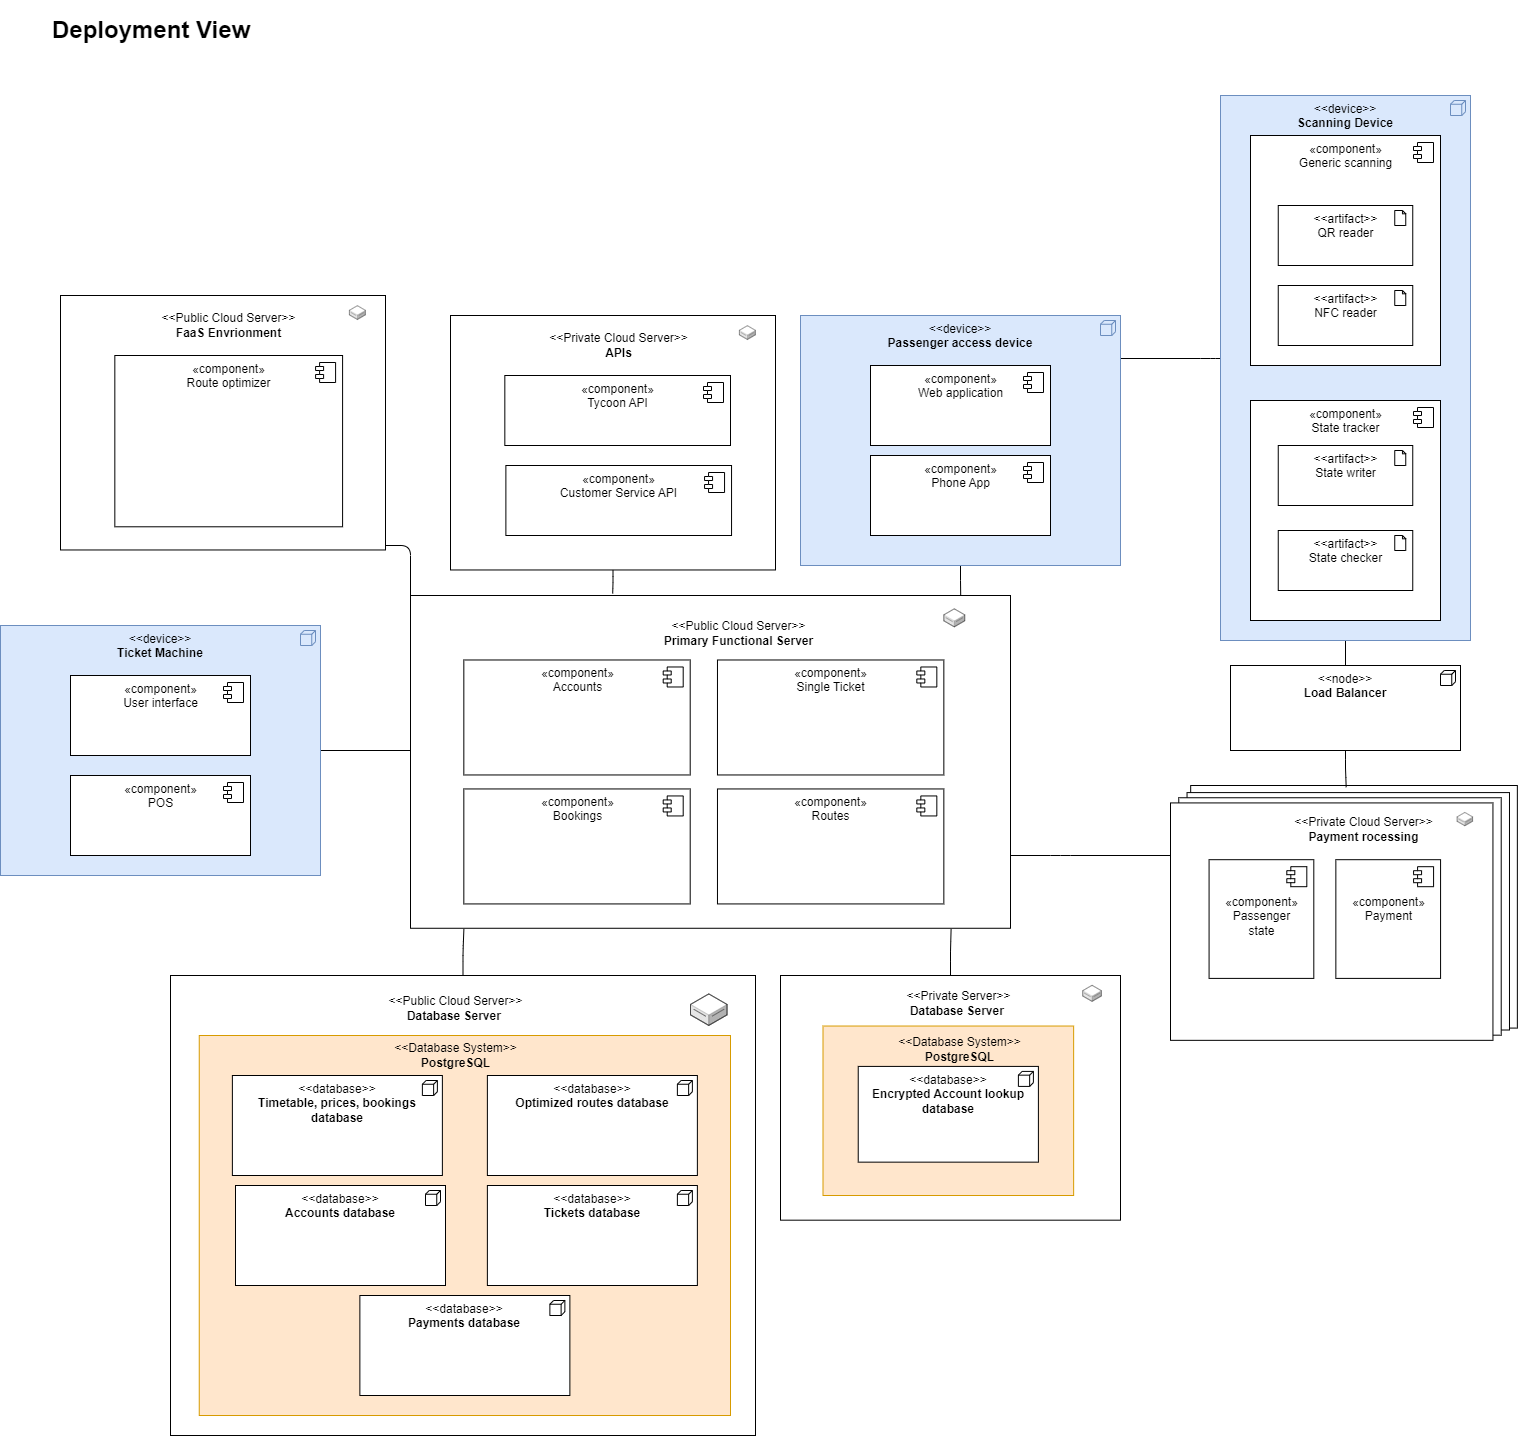
\includegraphics[width=\textwidth]{drawings/views_final_version/deployment_view.png}
    \caption{Deployment view related to the scanning procedure.}
    \label{fig:deployment_view_scanning}
\end{figure}

\subsubsection{Description}
The deployment view diagram illustrates the TrIP system's architecture, showing components distributed across public and private cloud servers. Public cloud servers house the FaaS Environment for route optimization, a Terminal with Customer Service API, and the Primary Functional Server hosting Accounts, Single Ticket, Bookings, and Routes components. Devices for passenger access, such as web and phone apps, interface with scanning devices like QR and NFC readers, managed by state trackers and checkers.

The ticket machine interfaces include User Interface and POS components. Database servers in the public cloud manage the PostgreSQL databases for Timetables, Prices, Bookings, Optimized Routes, Accounts, Tickets, and Payments. The private cloud server secures the Encrypted Account Lookup database. A Load Balancer ensures efficient traffic management.

Payment processing, crucial for managing Passenger State and payments, is securely handled in the private cloud, emphasizing the system's focus on security and reliable transaction handling. 
\subsubsection{Glossary of Elements}

\begin{table}[H]
    \centering
    \caption{Glossary for the Deployment View of the TrIP SYSTEM.}
    \label{tab:deployment_view_glossary}
    \begin{tabularx}{\textwidth}{@{}lXX@{}} % Corrected to have three columns
    \toprule
    \textbf{Component} & \textbf{Description} & \textbf{Hosted On} \\
    \midrule
    FaaS Environment & Provides a platform for executing backend functions in a serverless architecture, such as route optimization. & Public Cloud Servers \\
    Tycoon API & Interfaces allowing tycoons' software and systems to communicate with the TrIP system. & Private Cloud Servers \\
    Customer Service API & Facilitates customer service operations by providing data access and manipulation capabilities. & Private Cloud Servers \\
    Passenger Access Device & Equipment that passengers interact with to access the system, like ticket validation and purchases. & Terminal, App, Website \\
    Ticket Machine & Physical machines where passengers can purchase tickets and manage their bookings. & Station Locations \\
    Scanning Device & Tools used for reading ticket information, necessary for entry validation and passenger tracking. & Entry/Exit Gates \\
    QR Reader & Specialized scanners that interpret QR codes on tickets for entry validation or information retrieval. & Scanning Devices \\
    NFC Reader & Contactless devices that read NFC tags for authentication and ticket validation. & Passenger Access Devices \\
    Timetable, Prices, Bookings Database & Stores all relevant data for scheduling, pricing, and passenger bookings. & Public Cloud Servers \\
    Optimized Routes Database & Contains data on the most efficient routes calculated by the optimization algorithms. & Public Cloud Servers \\
    Accounts Database & Manages passenger account information, including subscription details and personal data. & Public Cloud Servers \\
    Tickets Database & Holds data related to ticket sales, validations, and historical transactions. & Public Cloud Servers \\
    Payments Database & Processes and records all payment transactions within the system. & Public Cloud Servers \\
    Encrypted Account Lookup Database & A secure database that stores sensitive account information, accessible only through authorized queries. & Private Cloud Servers \\
    \bottomrule
    \end{tabularx}
\end{table}
\subsubsection{Analysis on Perspectives}

\paragraph{Scenarios}
% Scenario: Upgrading Cloud Infrastructure for High Demand
\begin{table}[H]
    \centering
    \begin{tabularx}{\textwidth}{@{} lX @{}}
    \toprule
    \textbf{Aspect} & \textbf{Details} \\
    \midrule
    Source & TrIP system experiencing a surge in demand due to a new university opening at a station. \\
    Stimulus & Passenger numbers have more than quadrupled, causing performance delays during rush hours. \\
    Artifact & The deployment of the TrIP system across public cloud servers and private cloud servers. \\
    Response & The system's cloud infrastructure is updated to leverage elastic scaling capabilities. Load balancers distribute the increased traffic efficiently, and additional computing resources are allocated to handle the high load, particularly for route optimization and payment processing components. \\
    Measure & Post-update, the TrIP system handles a fourfold increase in user load with response times reduced by 70\%, ensuring that all passengers complete their transactions and receive route information within 2 seconds, even during peak rush hours. \\
    \bottomrule
    \end{tabularx}
    \caption{Scenario for Performance - Cloud Infrastructure Scaling}
    \label{table:performance_scaling}
\end{table}

% Scenario: Reinforcement of Data Security and Privacy Protocols
\begin{table}[H]
    \centering
    \begin{tabularx}{\textwidth}{@{} lX @{}}
    \toprule
    \textbf{Aspect} & \textbf{Details} \\
    \midrule
    Source & TrIP system architecture analysis in response to a competitor's security breach. \\
    Stimulus & The need to verify and bolster the security measures in place to protect passenger data. \\
    Artifact & Deployment architecture of the TrIP system with a focus on data servers and encryption protocols. \\
    Response & The system utilizes advanced encryption for data at rest and in transit within private cloud servers. Access controls are strictly enforced, ensuring only authenticated and authorized components interact with sensitive data. Periodic security audits and real-time intrusion detection systems are in place to monitor and immediately respond to any unauthorized access attempts. \\
    Measure & Security tests confirm no data leakage, and the system's compliance with the latest privacy regulations is validated by a third-party security firm, ensuring that the board and tycoons have verifiable assurance of the system's security measures. \\
    \bottomrule
    \end{tabularx}
    \caption{Scenario for Security - Privacy and Data Protection}
    \label{table:security_privacy}
\end{table}


In the Deployment Viewpoint, the TRiP system's architecture is strategically distributed across a combination of cloud-based and localized servers to optimize for both performance and security, critical attributes for the robustness and reliability of the system.

The TRiP system's deployment on cloud servers is engineered to enhance performance. The public cloud servers provide a scalable Fast Environment for handling dynamic user demands and instantaneous Route Optimization, ensuring that the most efficient paths are always available to the user. This optimization is further supported by Load Balancers, which are essential in managing network traffic by distributing workloads evenly, thereby preventing any server from becoming a bottleneck and ensuring a smooth user experience. 

For security, the system employs private cloud servers, where sensitive components such as the Encrypted Account Lookup Database are hosted. The encryption of this database is a crucial security measure, safeguarding personal and travel data against unauthorized access. 

% Scenario 1: Usability Enhancement through Standardized UIs
% Scenario: Efficient Data Retrieval for Tycoon Route Analysis and Account Information
\begin{table}[H]
    \centering
    \begin{tabularx}{\textwidth}{@{} lX @{}}
    \toprule
    \textbf{Aspect} & \textbf{Details} \\
    \midrule
    Source & Tycoon's analytical system requesting data for route pricing and passenger account details. \\
    Stimulus & The Tycoon system sends a data request to analyze route prices based on their subscription models and to gather specific account information for passengers. \\
    Artifact & Tycoon API interfacing between the Tycoon's systems and the TrIP system's databases. \\
    Response & The Tycoon API promptly routes the queries to the appropriate data providers, retrieves the requested information, and consolidates the results for the Tycoon system. \\
    Measure & Tycoon system receives comprehensive data within 3 seconds, enabling effective route and subscription analysis for passenger accounts. \\
    \bottomrule
    \end{tabularx}
    \caption{Scenario for Tycoon API Data Retrieval}
    \label{table:tycoon_api_data_retrieval}
\end{table}

% Scenario: Streamlined System Updates through MVC Pattern
\begin{table}[H]
    \centering
    \begin{tabularx}{\textwidth}{@{} lX @{}}
    \toprule
    \textbf{Aspect} & \textbf{Details} \\
    \midrule
    Source & TrIP system development team. \\
    Stimulus & The need to update the route pricing algorithm without affecting the user interface. \\
    Artifact & Model-View-Controller (MVC) pattern within the TrIP system. \\
    Response & Developers update the Pricing Model with the new algorithm, which automatically propagates changes to the relevant Views without requiring additional adjustments. \\
    Measure & The system update is deployed with zero downtime, and subsequent feature updates require 40\% less time due to decoupled architecture. \\
    \bottomrule
    \end{tabularx}
    \caption{Scenario for Maintainability - MVC Pattern}
    \label{table:mvc_maintainability}
\end{table}

% Scenario: Enhanced User Experience with MVC-Driven UI
\begin{table}[H]
    \centering
    \begin{tabularx}{\textwidth}{@{} lX @{}}
    \toprule
    \textbf{Aspect} & \textbf{Details} \\
    \midrule
    Source & Passenger using the TrIP system to manage travel. \\
    Stimulus & The passenger updates their travel preferences in the User Account View. \\
    Artifact & MVC pattern facilitating the User Account management. \\
    Response & The Controller processes the passenger's input, updates the User Account Model, and the View dynamically reflects the changes, providing immediate visual confirmation to the passenger. \\
    Measure & Passengers express a 90\% satisfaction rate with the ease of updating preferences, and the error rate in preference updates decreases by 50\%. \\
    \bottomrule
    \end{tabularx}
    \caption{Scenario for Usability - MVC-Driven UI}
    \label{table:mvc_usability}
\end{table}


\section{Development Viewpoint}
We start discussing the information viewpoint by analyzing stakeholder concerns that need to be addressed.
We individuated the following user stories:
\begin{itemize}
    \item User stories TODO
\end{itemize}

As a consequence, we decided to prioritize Quality Attributes for this view as indicated in Table~\ref{tab:development_view}.
\begin{table}[h!]
    \centering
    \resizebox{\textwidth}{!}{%
    \begin{tabular}{|l|c|c|c|c|c|c|c|c|c|}
      \hline
      & Usability & Performance & Security & Modifiability & Cost Efficiency & Availability & Safety & Integrability & Maintainability \\
      \hline
      Development View & 
      \cellcolor{gray!60}X & % Usability (2nd priority)
       & % Performance
       & % Security
       \cellcolor{gray!40}X& % Modifiability
       & % Cost Efficiency
       & % Availability
       & % Safety
       \cellcolor{gray!25}X& % Integrability
      \cellcolor{gray!90}X \\ % Maintainability (1st priority)
      \hline
    \end{tabular}
    }
    \caption{Development View Prioritized Quality Attributes}
    \label{tab:development_view}
\end{table}

\subsection{View: Broker pattern for Tycoon API}
\subsubsection{Model}
\begin{figure}[H]
    \centering
    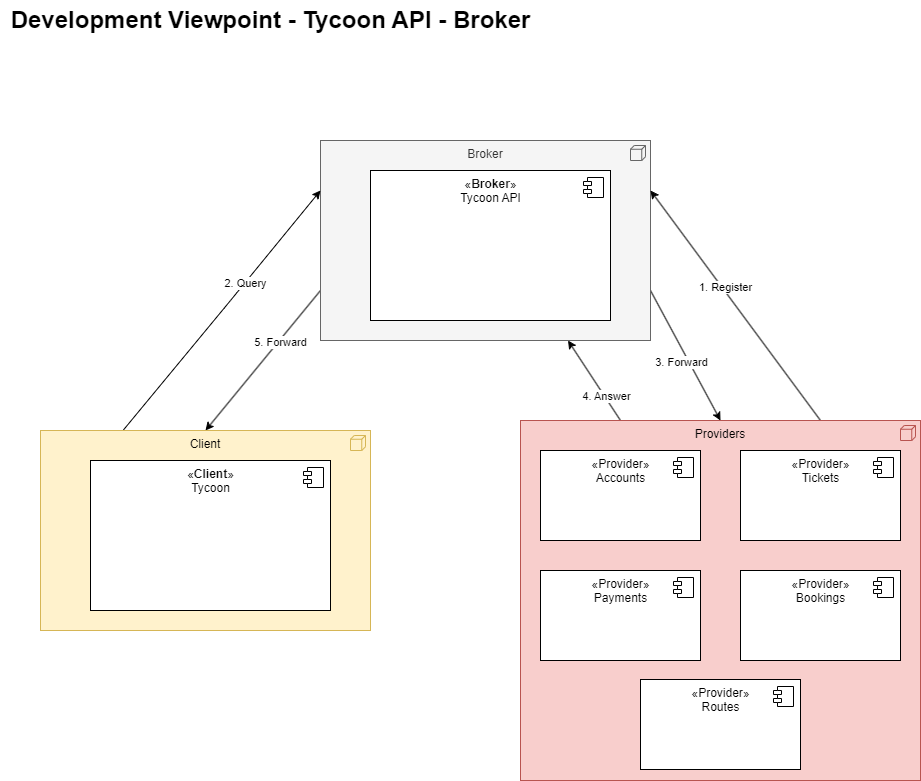
\includegraphics[width=\textwidth]{drawings/views_final_version/development_view_broker.png}
    \caption{Deployment view related broker pattern related to Tycoon API.}
    \label{fig:development_view_broker}
\end{figure}
\subsubsection{Description}
The diagram portrays the broker architecture in the TrIP system, delineating the communication between clients, the broker, and providers. Tycoon clients initiate the interaction by registering with the Tycoon API broker. Queries are sent from the Tycoon to the broker, which then forwards these queries to the relevant providers. These providers include services for Accounts, Payments, Bookings, Tickets, and Routes, each playing a pivotal role in processing Tycoon requests. Upon gathering the necessary data or performing the required actions, providers send their response back to the broker. The broker, in turn, forwards this information back to the Tycoon client, completing the request-response cycle. This broker pattern facilitates a structured approach to handling requests and centralizes the communication logic, simplifying interactions across the system’s diverse components.
\subsubsection{Glossary of Elements}

\begin{table}[H]
    \centering
    \caption{Glossary for the Broker in the Development View.}
    \label{tab:broker_development_glossary}
    \begin{tabular}{@{}llp{10cm}@{}}
        \toprule
    \textbf{Id} & \textbf{Name} & \textbf{Description} \\
    \midrule
    1 & Client & Represents the Tycoon requesting data or action from the broker. \\
    2 & Broker & Tycoon API that mediates between clients (Tycoon's) and various service providers (TrIP System's modules), handling requests and responses. \\
    3 & Provider & TrIP system that register with the broker to offer their services to clients. \\
    4 & Tycoon API & The application programming interface provided by the broker for communication with clients and providers. \\
    5 & Query & A request sent from the client to the broker, seeking information or action. \\
    6 & Register & The action of a provider adding their services to the broker's list of available resources. \\
    7 & Forward & The process of the broker sending requests to providers or responses back to clients. \\
    8 & Answer & The provider's response to a query that is sent back to the client via the broker. \\
    9 & Accounts & TrIP System module that manages user account information and authentication. \\
    10 & Tickets & TrIP system for issuing tickets, usually related to events or transportation. \\
    11 & Payments & The TrIP module that handles transaction processing. \\
    12 & Bookings & TrIP System module that manages reservations for services offered by the provider. \\
    13 & Routes & TrIP System module that handles route pricing. \\
    \bottomrule
    \end{tabular}
\end{table}
\subsubsection{Analysis on Perspectives}
\paragraph{Scenarios}
\scenarioOneDevelopment

\subsection{View: Model-View-Controller pattern for User Interface}
\subsubsection{Model}
\begin{figure}[H]
    \centering
    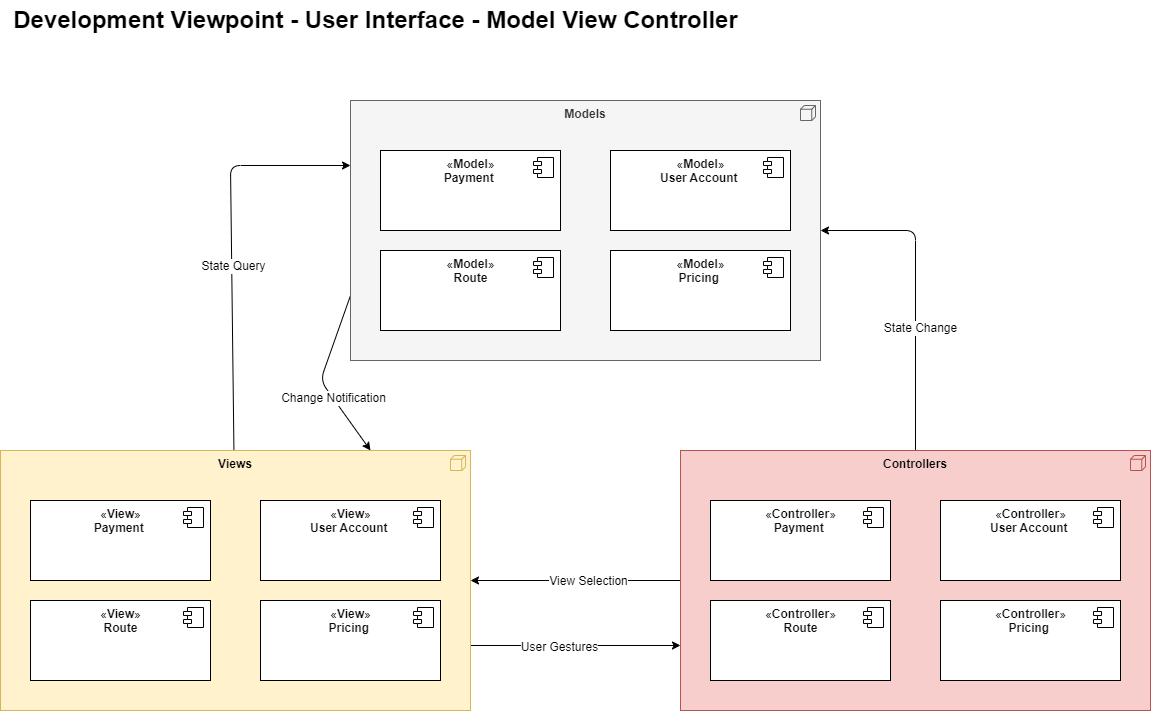
\includegraphics[width=\textwidth]{drawings/views_final_version/development_view_User_Interface.png}
    \caption{Development view model-view-controller pattern for UI}
    \label{fig:development_view_User_Interface}
\end{figure}

\subsubsection{Description}
This diagram illustrates the Model-View-Controller (MVC) pattern applied within the TrIP system. It breaks down the system's user interface into Views, which are responsible for presenting data to users and include interfaces for Payment, User Account, Route, and Pricing. The Models act as the data layer with Payment, Route, User Account, and Pricing components that manage the system's state. They receive state queries and broadcast state changes to the Views. Controllers interpret user gestures, direct state changes, and mediate between the Models and Views. This separation of concerns ensures that user interactions are handled efficiently, system data is managed cohesively, and business logic is executed in a controlled manner. The MVC architecture is fundamental to the system's organization, promoting clear delineations between different functionalities and facilitating ease of maintenance and scalability.

\subsubsection{Glossary of Elements}

\begin{table}[H]
    \centering
    \caption{Legend for the User Interface Components in the Development View of the TrIP System.}
    \label{tab:trip_system_ui_development_legend}
    \begin{tabular}{@{}llp{10cm}@{}}
    \toprule
    \textbf{Id} & \textbf{Name} & \textbf{Description} \\
    \midrule
    1 & Views & User interface components of the TrIP system that passengers interact with, including elements like payment, account management, and route selection screens. \\
    2 & Models & Data structures in the TrIP system that encapsulate the core business logic related to payment, user accounts, route information, and pricing. \\
    3 & Controllers & Components within the TrIP system that manage input from passengers, process requests, and produce responses by interacting with Models and updating Views. \\
    4 & Payment View/Model/Controller & Dedicated interfaces, data, and logic for processing passenger payments within the TrIP system, ensuring secure transactions. \\
    5 & User Account View/Model/Controller & Elements responsible for managing passenger profiles, including authentication and handling of personal account details in the TrIP system. \\
    6 & Route View/Model/Controller & Components that handle the presentation, data management, and operational logic of travel routes available to passengers in the TrIP system. \\
    7 & Pricing View/Model/Controller & The set of user interfaces, algorithms, and data that determine and manage fare calculations and display pricing information to passengers. \\
    8 & State Query & A request by the TrIP system to retrieve the current state, such as checking a passenger's account status or ticket validity. \\
    9 & State Change & An update within the TrIP system that alters the current state in response to passenger actions or other operational changes. \\
    10 & Change Notification & A notification mechanism that informs the TrIP system and passengers when a significant change has occurred, such as a payment confirmation or route update. \\
    11 & User Gestures & Interactions by passengers with the TrIP system, like touch or click actions, which are interpreted as commands to navigate or provide input. \\
    12 & View Selection & The process within the TrIP system for choosing the appropriate user interface view to display to passengers based on the current context or request. \\
    \bottomrule
    \end{tabular}
\end{table}

\subsubsection{Analysis on Perspectives}
\paragraph{Scenarios}
\scenarioTwoDevelopment
\scenarioThreeDevelopment

The Development Viewpoint focuses on the structural aspects that underpin the TrIP system's architecture, highlighting the modular approach in system design to enhance usability and maintainability. \\

\noindent \textbf{MVC Pattern:} \\
The adoption of the Model-View-Controller (MVC) pattern substantially improves the system's maintainability by segregating the user interface elements (Views) from the business logic (Models) and user input processing (Controllers). This separation of concerns allows developers to update or modify one aspect of the system — such as adding new features to the user interface — without the need to alter the underlying business logic or control flow. For passengers, this results in a more comprehensive interface with a variety of options and features, enhancing the overall usability of the system. The MVC pattern ensures that as passenger needs evolve, new Views can be added swiftly, making the system both adaptable and future-proof. \\

\noindent \textbf{Broker Architecture:} \\
In parallel, the broker architecture employed within the Tycoon API streamlines the interaction process between the Tycoons and the TrIP system. It serves as a centralized point for processing queries and handling communications, thus simplifying the complexity of these interactions. For the Tycoons, this architecture means usability is significantly enhanced, allowing them to communicate through a unified interface with the Tycoon API, which abstracts the intricate workings of the TrIP system's service modules. This consolidation of communication logic not only benefits the Tycoons but also reduces the overhead for the TrIP system in managing multiple communication protocols. \\

These architectural decisions, reflected in the Development Viewpoint, are key to the TrIP system's ability to offer an efficient, secure, and user-friendly platform that can grow and adapt in line with technological advancements and user expectations.


\appendix

\section{User Stories}

\subsection{Prioritized User Stories}
The prioritization of selected user stories focuses on core objectives such as enhancing passenger experience, ensuring security, promoting operational efficiency, and facilitating seamless integration:

\begin{itemize}
    \item \textbf{User Stories 1 and 16} simplify the payment process, enhancing usability and convenience across multiple networks.
    \item \textbf{User Story 18} secures personal and financial data, aligning with trust-building and regulatory compliance.
    \item \textbf{User Story 29} underlines operational cost-efficiency, vital for the system's sustainability.
    \item \textbf{User Story 23} ensures smooth integration with existing railroad infrastructure, key to operational continuity and adoption.
    \item \textbf{User Stories 4 and 7} use technology to improve accessibility and the user experience, making the system inclusive.
    \item \textbf{User Stories 26 and 27} highlight adaptability in maintenance and scheduling, crucial for service quality and minimizing passenger disruption.
\end{itemize}

Prioritizing these stories ensures the system meets crucial user needs and operational objectives, setting a foundation for success and growth.

\subsection{Passengers}
\begin{itemize}
    \item \userStoryOne
    \item \userStoryTwo
    \item \userStoryThree
    \item \userStoryThirtySeven
    \item \userStoryThirtyNine
\end{itemize}

\subsection{Tech-savvy Passengers}
\begin{itemize}
    \item \userStoryFour
    \item \userStoryFive
\end{itemize}

\subsection{Accessibility Advocates}
\begin{itemize}
    \item \userStorySix
    \item \userStorySeven
    \item \userStoryEight
    \item \userStoryNine
    \item \userStoryTen
\end{itemize}

\subsection{Passengers with Special Considerations}
\begin{itemize}
    \item \userStoryEleven
    \item \userStoryTwelve
    \item \userStoryThirteen
    \item \userStoryFourteen
    \item \userStoryFifteen
    \item \userStorySixteen
    \item \userStorySeventeen
\end{itemize}

\subsection{Government}
\begin{itemize}
    \item \userStoryEighteen
    \item \userStoryNineteen
    \item \userStoryTwenty
\end{itemize}

\subsection{Tycoons (Train Company Owners)}
\begin{itemize}
    \item \userStoryTwentyOne
    \item \userStoryTwentyTwo
    \item \userStoryTwentyThree
    \item \userStoryTwentyFour
    \item \userStoryThirtyFive
    \item \userStoryThirtyEight
    \item \userStoryForty
\end{itemize}

\subsection{Financial Analysts}
\begin{itemize}
    \item \userStoryTwentyFive
\end{itemize}

\subsection{Station Staff}
\begin{itemize}
    \item \userStoryTwentySix
\end{itemize}

\subsection{Maintenance Teams}
\begin{itemize}
    \item \userStoryTwentySeven
\end{itemize}

\subsection{Government Financial Auditors}
\begin{itemize}
    \item \userStoryTwentyEight
\end{itemize}

\subsection{TrIP Owner}
\begin{itemize}
    \item \userStoryFortyOne
    \item \userStoryTwentyNine
    \item \userStoryThirty
    \item \userStoryThirtyOne
    \item \userStoryThirtyTwo
    \item \userStoryThirtyThree
    \item \userStoryThirtyFour
\end{itemize}

\subsection{System administrator}
\begin{itemize}
    \item \userStoryThirtySix
\end{itemize}

% \begin{table}[H]
    \resizebox{\textwidth}{!}{%
    \begin{tabular}{|l|c|c|c|c|c|c|c|c|c|c|c|}
    \hline
    \textbf{User Story} & \textbf{Usability} & \textbf{Performance} & \textbf{Security} & \textbf{Modifiability} & \textbf{Deployability} & \textbf{Energy Efficiency} & \textbf{Availability} & \textbf{Safety} & \textbf{Integrability} & \textbf{Testability} & \textbf{Accessibility} \\
    \hline
    1. Frequent traveler monthly pass & + &  &  &  &  &  &  &  &  &  &  \\
    \hline
    2. Check travel card balance & + &  &  &  &  &  &  &  &  &  &  \\
    \hline
    3. Subscription notifications & + &  &  &  &  &  &  &  &  &  &  \\
    \hline
    4. Mobile app management & + &  &  &  & - &  &  &  &  &  &  \\
    \hline
    5. Carbon footprint tracking &  & - &  &  &  & + &  &  &  &  &  \\
    \hline
    6. Accessible services info & + &  &  &  &  &  &  & + &  &  &  \\
    \hline
    7. Voice-activated features & + &  &  & - & - &  &  &  &  &  & + \\
    \hline
    8. Simple interface for elders & + &  &  & + &  &  &  &  &  &  &  \\
    \hline
    9. Multilanguage options & + &  &  & - &  &  &  &  &  &  &  \\
    \hline
    10. Quick access to popular trips & + & - &  & - &  &  &  &  &  &  &  \\
    \hline
    11. Scan student card for benefits & + &  &  & - &  &  &  &  &  &  &  \\
    \hline
    12. Single transaction for subscriptions & + & - &  &  &  &  &  &  &  &  &  \\
    \hline
    13. Charge train cards at terminal & + &  &  & - &  &  &  &  &  &  &  \\
    \hline
    14. Interface for visually impaired & + &  &  &  &  &  &  &  &  &  & + \\
    \hline
    15. Block payment for blocked routes & + & - &  & - &  &  &  &  &  &  &  \\
    \hline
    16. Single ticket across all networks & + & - &  & - &  &  &  &  &  &  &  \\
    \hline
    17. Subscriptions advice for commuting & + & - &  & - &  &  &  &  &  &  &  \\
    \hline
    18. Adherence to security standards &  &  & + & - &  &  &  &  & - & - &  \\
    \hline
    19. Detailed reporting for government & + &  &  & - &  &  &  &  & - &  &  \\
    \hline
    20. Reduced fares for eligible populations & + & - &  & - &  &  &  &  &  &  &  \\
    \hline
    21. Revenue tracking for tycoons & + & - &  & - &  &  &  &  &  &  &  \\
    \hline
    22. Exclusive promotions & + &  &  & - &  &  &  &  &  &  &  \\
    \hline
    23. Payment system integration & + &  &  & - &  &  &  &  & + & - &  \\
    \hline
    24. Access to analytics &  &  &  & - &  &  &  &  & + &  &  \\
    \hline
    25. Assistance for ticket purchases & + &  &  & - &  &  &  &  &  &  &  \\
    \hline
    26. Temporary fare adjustments &  &  &  & - &  & + &  &  &  &  &  \\
    \hline
    27. Integration with maintenance tools &  &  &  & - &  & + &  &  &  &  &  \\
    \hline
    28. Audit trails and compliance &  &  &  & - &  &  &  &  &  &  &  \\
    \hline
    \end{tabular}%
    }
    \caption{User Stories and Quality Attributes}
\end{table}

\section{Stakeholder Priorities by Events}

\begin{table}[htbp]
\centering
\caption{Event Updates for Stakeholder Requirements for the TrIP System}
\begin{tabular}{
  >{\raggedright\arraybackslash}p{2.5cm}
  >{\raggedright\arraybackslash}p{3.5cm}
  >{\raggedright\arraybackslash}p{3.5cm}
  >{\raggedright\arraybackslash}p{3.5cm}
  >{\raggedright\arraybackslash}p{3.5cm}
}
\toprule
\textbf{Stakeholder} & 
\textbf{Initial QA Priorities} & 
\textbf{Event 1: New Tycoons} & 
\textbf{Event 2: Unreliable Network} & 
\textbf{Event 3: Traffic Jams} \\
\midrule
TrIP Owner & 
Maintainability (2), Operational Costs (2) & 
\cellcolor{changeColor}\makecell[tl]{Scalability (2)} & 
\cellcolor{changeColor}\makecell[tl]{Availability (2) \\ Maintainability (1) \\ Cost (1) } & 
\makecell[tl]{\textit{No new change}} \\
\midrule
Tycoons & 
Usability (1), Reliability (2) & 
\makecell[tl]{\textit{No new change}} & 
\makecell[tl]{\textit{No new change}} & 
\cellcolor{changeColor}\makecell[tl]{Performance (3)} \\
\midrule
Passengers & 
Usability (2), Security (1) & 
\makecell[tl]{\textit{No new change}} & 
\makecell[tl]{\textit{No new change}} & 
\makecell[tl]{\textit{No new change}} \\
\midrule
\multicolumn{5}{c}{\textbf{Event 4: Data Leaks}} \\
\cmidrule{2-5}
TrIP Owner & 
\multicolumn{4}{l}{\cellcolor{changeColor}\makecell[tl]{Security (2)}} \\
\cmidrule{2-5}
Railroad Tycoons & 
\multicolumn{4}{l}{\makecell[tl]{\textit{No new change}}} \\
\cmidrule{2-5}
Passengers & 
\multicolumn{4}{l}{\makecell[tl]{\textit{No new change}}} \\
\bottomrule
\end{tabular}
\end{table}

    



\end{document}
